\lettrine{I}{n this chapter}, we present and discuss the results of our study. We present statistical evaluations for each of the tests that we outlined in Chapter~\ref{chap_investigation}. Note that the evaluations are mostly based on the complement sizes resulting from the different constructions. As mentioned, the complement size is our main performance measure, and the execution time is a secondary one (because it is not perfectly repeatable and comparable). We present a part of the measured execution times in this chapter (namely, from the Michel test set), however, the rest of the execution times can be found in Appendix~\ref{app_times}.

In Section~\ref{5_internal}, we present the results of the internal tests, and in Section~\ref{5_external}, the results of the external tests. Both sections treat the results for the \goal{} test set and the Michel test set separately. In Section~\ref{5_discussion} we present the discussion of the results, including a result summary, the gained insights, and the limitations of the stduy.


\section{Results of the Internal Tests}
\label{5_internal}
The goal of the internal tests is to test different versions of the Fribourg constructions and to compare their results against each other. Below, we first present the results of the internal tests on the \goal{} test set (Section~\ref{5_internal_goal}), and then the results of the internal tests on the Michel test set (Section~\ref{5_internal_michel}).

\subsection{GOAL Test Set}
\label{5_internal_goal}
For the \goal{} test set, the tested versions of the Fribourg construction are the following (see Section~\ref{4_internal}):

\begin{enumerate}
\item Fribourg
\item Fribourg+R2C
\item Fribourg+R2C+C
\item Fribourg+M1
\item Fribourg+M1+R2C
\item Fribourg+M1+R2C+C
\item Fribourg+M1+M2
\item Fribourg+R
\end{enumerate}

Below we present the results for all these eight versions from different perspectives. First, we determine the effective samples, on which the rest of he analysis is based. Then, we first analyse the results aggregated over the entire test set, and then split up by the 110 transition density/acceptance density classes of the \goal{} test set. Finally, we try to generalise these per-class results by establishing a categorisation of the \goal{} test set into \textit{easy}, \textit{medium}, and \textit{hard} classes.

\subsubsection{Effective Samples}
First of all, we have to check how many timeouts and memory excesses there are in order to establish the effective samples, that is, the set of automata that have been successfully complemented by \textit{all} of the tested constructions.All the remaining analyses in this section are based on this set of effective samples. Table~\ref{i.g.out_table} shows the number of timeouts and memory excesses for each of the tested Fribourg construction versions.

\begin{table}[ht]
\centering
% latex table generated in R 3.1.2 by xtable 1.7-4 package
% Sat Jun  6 16:42:17 2015
\begin{tabular}{lrr}
  \hline
Construction & Timeouts & Memory excesses \\ 
  \hline
Fribourg & 48 & 0 \\ 
  Fribourg+R2C & 30 & 0 \\ 
  Fribourg+R2C+C & 54 & 0 \\ 
  Fribourg+M1 & 2 & 0 \\ 
  Fribourg+M1+M2 & 1 & 0 \\ 
  Fribourg+M1+R2C & 1 & 0 \\ 
  Fribourg+M1+R2C+C & 8 & 0 \\ 
  Fribourg+R & 48 & 0 \\ 
   \hline
\end{tabular}

\caption{Number of timeouts and memory excesses in the internal tests on the \goal{} test set.}
\label{i.g.out_table}
\end{table}

As can be seen in Table~\ref{i.g.out_table}, there is no memory excess for any of the constructions. That is, none of the constructions required more than 1 GB Java heap for any of the 11,000 complementation tasks in the \goal{} test set. However, as can be seen, there are some timeouts. For example, Fribourg, has 48 timeouts, which means that 48 of its complementation tasks were aborted, because they exceeded the time limit of 600 CPU time seconds per automaton.

Based on these results, we have to determine the effective samples, that is, the set of automata that have been successfully processed by \textit{all} the eight constructions. The analysis yields a set of effective samples of 10,939 automata. This means that 61 automata (0.55\%) are excluded because their complementation failed for at least one of the constructions. All the following analyses will be based on these 10,939 automata.

\subsubsection{Overall Results}
Having determined the effective samples, we can turn to the analysis of our main performance measure, the sizes of the produced complements. To get a first impression, in Figure~\ref{i.g.stripchart} we plot all the measured complement sizes in a stripchart. The complement sizes of all the tested constructions are represented as a strip containing a circle for each of the 10,939 automata of the effective samples. The number of states of the corresponding complements are indicated on the $x$-axis.

\begin{figure}[ht]
\centering
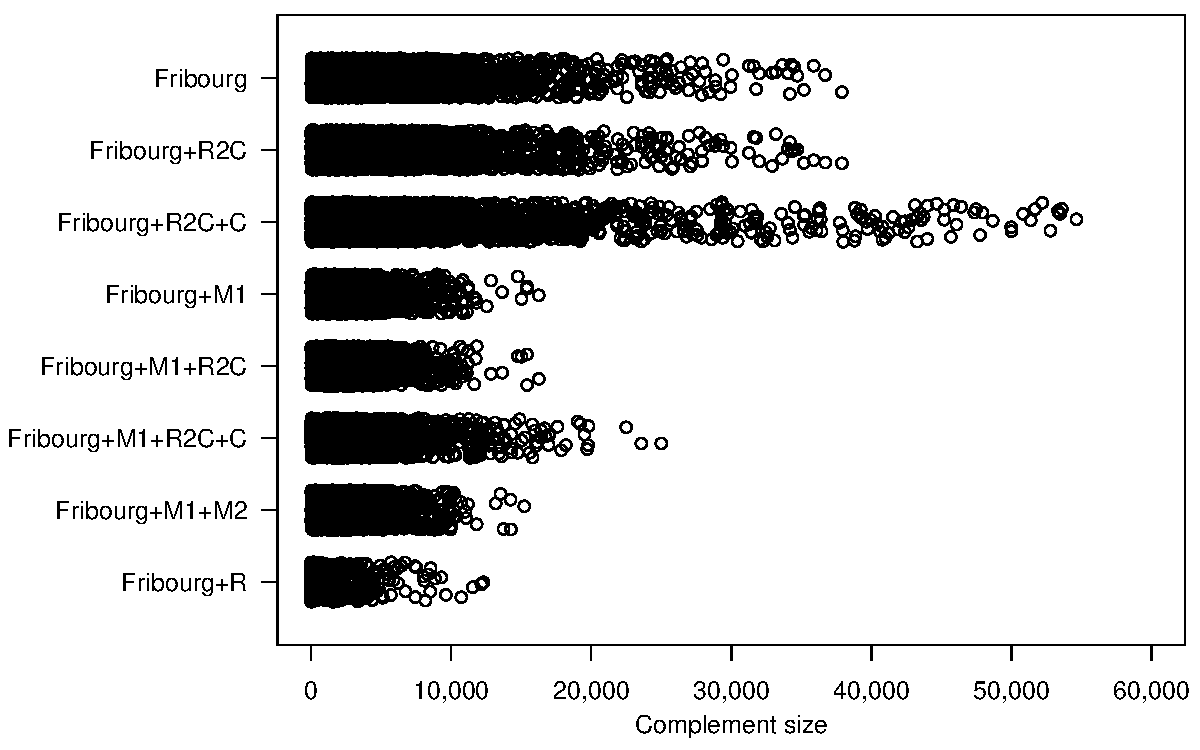
\includegraphics[scale=0.575]{figures/r/internal/goal/s.stripchart.pdf}
\caption{Complement sizes of the 10,939 effective samples for each tested version of the Fribourg construction on the \goal{} test set.}
\label{i.g.stripchart}
\end{figure}

The first thing to note is that the distribution of complement sizes is right-skewed (also known as positive-skewed). This means that there are many small complements, and then gradually fewer larger complements. This results in a long tail toward the right  on the $x$-axis. Generally, in right-skewed distributions, the mean is larger than the median, because the mean is increased by the few number of larger or extremely large values. We will see that this is the case for our complement size distribution below.

The stripchart allows to intuitively compare the density of large complements that are produced by the different versions. Going from top to bottom, the distributions of Fribourg and Fribourg+R2C have similarly long tails. Fribourg+R2C+C, however, has a considerably longer tail. This shows us that the C option has a significant effect on the complement sizes, because it adds an additional state to the automata which are not complete. As we have seen in Section~\ref{4_goal_testset}, only 9\% of the automata of the \goal{} test set are already complete. Thus 91\% of the automata are affected by the C option.

Next, Fribourg+M1, Fribourg+M1+M2, and Fribourg+M1+R2C all have similarly long tails. However, these tails are significantly shorter than the ones of the previous three versions. This indicates that the M1 optimisation is very effective in reducing the complement sizes.

Fribourg+M1+R2C+C again has a longer tail than Fribourg+M1+R2C. The reason for this is most likely the effect of the C option that we already observed for Fribourg+R2C and Fribourg+R2C+C.

Finally, Fribourg+R has the shortest tail of all versions. Fribourg+R is a special case, because it is the same construction as Fribourg, but with the difference that at the end of the construction, all unreachable and dead states are removed. Comparing the strips of Fribourg and Fribourg+R thus gives an idea of how many unreachable and dead states the Fribourg construction produces for the tested automata.

The stripchart in Figure~\ref{i.g.stripchart} gives a good first impression about the distribution of produced complement sizes of the different versions. However, for further insights, we need to statistically evaluate these distributions. Table~\ref{i.g.stats} shows the mean complement size for each version, along with the classical five-number summary consisting of the minimum value, 25th percentile, median, 75th percentile and maximum value.

\begin{table}[ht]
\centering
% latex table generated in R 3.1.2 by xtable 1.7-4 package
% Sat Jun  6 16:42:20 2015
\begin{tabular}{lrrrrrr}
  \hline
Construction & Mean & Min. & P25 & Median & P75 & Max. \\ 
  \hline
Piterman+EQ+RO & 209.6 & 1 & 38.0 & 80.0 & 183.0 & 20,349 \\ 
  Slice+P+RO+MADJ+EG & 949.4 & 2 & 120.0 & 396.0 & 1,003.0 & 41,081 \\ 
  Fribourg+M1+R2C & 1,017.3 & 2 & 153.0 & 452.0 & 1,134.0 & 37,068 \\ 
   \hline
\end{tabular}

\caption{Statistics of the complement sizes of the 10,939 effective samples for each tested version of the Fribourg construction on the \goal{} test set.}
\label{i.g.stats}
\end{table}

As can be seen in Table~\ref{i.g.stats}, the mean is for all constructions significantly higher than the median. This is typical for right-skewed distributions. Generally, the median is said to be more robust than the mean, because it is not affected by extreme values. For example, for the distribution $(1,2,3,4,5)$ the mean and the median are both 3. If this distribution happens to contain an extreme value, for example, $(1,2,3,4,1000)$, then the mean is increased to 202, while the median is still 3. Thus, the median better represents the ``typical'' values of a distribution, whereas the mean better reflects the effect of extreme values. Both aspects may be important for the analysis of the data at hand. For our own analyses, we will mainly focus on the median, because we are more interested in the ``typical'' behaviour of the tested constructions. However, we will always put the median in relation with the mean and the the other statistical indicators in Table~\ref{i.g.stats}.

The medians in Table~\ref{i.g.stats} include provide interesting insights. Fribourg has a median complement size of 761. This means that half of all the complements produced by Fribourg have 761 or fewer states, and the other half has more than 761 states. For Fribourg+R2C, the median decreases from 761 to 689. This is because the R2C optimisation removes states, whose rightmost component has colour 2, from the output automata. However, this applies only to the input automata which are complete, and as we determined in Section~\ref{4_goal_testset}, these are only 9\% of the \goal{} test set. Considering this, the R2C optimisation seems to be very effective in reducing complement sizes.

Regarding Fribourg+R2C+C the median complement size drops significantly to 451. This is surprising insofar as Fribourg+R2C+C has the highest mean of all versions, and in the stripchart in Figure~\ref{i.g.stripchart}, it has the longest tail. Thus at first glance, Fribourg+R2C+C might look like the version with the worst performance. However, regarding the median (as well as the 25th percentile) Fribourg+R2C+C belongs actually to the best versions. On the other hand, regarding the 75th percentile and the maximum, Fribourg+R2C+C has actually the highest values. A possible explanation for this is that the R2C+C option combination makes easy complementation tasks easier and hard complementation tasks harder. We will further elaborate on this point when analysing the median complement sizes separately for all the transition density/acceptance density classes. 

Regarding Fribourg+M1 and Fribourg+M1+M2, the median of Fribourg is lower than the median of the latter (482 against 496). The same applies to the 25th and 75th percentile. This means that the application of the M1 optimisation alone results in smaller complements than the application of the M1 and M2 optimisations together. At first sight this is surprising, because Fribourg+M1+M2 has a lower worst-case complexity than Fribourg+M1 (see Section~\ref{3_optimisations}). However, as we already hinted at in Section~\ref{1_empirical} in the introductory chapter, a lower worst-case state complexity does not mean smaller complements in concrete cases. With the results of Fribourg+M1 and Fribourg+M1+M2 we have an empirical evidence for this claim. Note that the mean of Fribourg+M1+M2 is slightly lower than the mean of Fribourg+M1, which might result from the cases where Fribourg+M1 produces larger complements than Fribourg+M1+M2. However, regarding the median, 25th percentile, and 75th percentile values, we still see Fribourg+M1 as the more performant version for the \goal{} test set, as we have indicated in Section~\ref{4_internal}.

Fribourg+M1+R2C decreases the median of Fribourg+M1 from 482 to 447. Also the 25th and 75th percentile are decreased. This results from the removal of states that the R2C option allows for the 9\% of complete automata in the \goal{} test set.

Comparing Fribourg+M1+R2C with Fribourg+M1+R2C+C, we observe a similar phenomenon as for Fribourg+R2C and Fribourg+R2C+C. The median and 25th percentile drop significantly, whereas the mean, 75th percentile, and maximum value increase. Again it seems that making the 91\% of incomplete automata preliminarily complete (by the C option) in order to apply the R2C optimisation to all of them, has a very positive effect on some automata, but a negative effect on others.

Finally, the results of Fribourg+R make apparent that this version is a special case. The median is 1, and further analysis reveals that all complements up to the 61st percentile have a size of 1. This number coincides well with the 61.8\% of automata in the \goal{} test set that are universal (see Section~\ref{4_goal_testset}). These universal automata indeed have a minimum complement consisting of a single non-accepting state (an empty automaton). It seems that whatever complement the Fribourg construction produces for these automata, the R option prunes all but one state. Even though universal automata are special cases, the results of Fribourg+R still give an idea about the number of unreachable and dead states that are produced by the Fribourg construction.

\subsubsection{Results by Transition Density/Acceptance Density Classes}
Up to now, we looked at the results that are aggregated over the entire test set. This mixes together all the automata of the 110 transition density/acceptance density classes. In the following, we analyse the results for each of these 110 classes separately. The goal is to reveal how the constructions perform on automata with very different characteristics, and to reveal the relative differences between them.

Such class-based analysis means that there is not just one value per statistical indicator for each construction, but 110 values, one for each class. For example, for every tested construction there are 110 means, 110 medians, and so on. In order to be able to present this amount of data, we restrict ourselves to the median values of each class. As already mentioned, our main focus is on the median, because it best reflects the ``typical'' results. Consequently, all the reported values in the following are median values. 

The per-class median complement sizes result in a similar type of data that we encountered in the analysis of the complete, universal, and empty automata in the \goal{} test set in Section~\ref{4_goal_testset}. There, we presented this data in two forms, as matrices and as perspective plots. The advantage of matrices is that they show the explicit values, the advantage of perspective plots is that they better show the relative differences and the overall pattern. For the sake of brevity, we use only perspective plots in this chapter. However, we provide the matrices corresponding to all the perspective plots of this chapter in Appendix~\ref{app_matrices}.

Figures~\ref{i.g.persp_1} and~\ref{i.g.persp_2} show the perspective plots with the per-class median complement sizes for the eight tested Fribourg construction version. Note that looking at these perspective plots corresponds to looking at the corresponding matrix from the bottom right corner. We keep this orientation for all the perspective plots in this chapter. Note that this orientation is different from the orientation used for the perspective plots presenting the number of complete, universal, and empty automata of the \goal{} test set in Section~\ref{4_goal_testset}. The colours of the rectangles (called facets) in the perspective plots depend on the ``height'' of the plot at their four corners, and are chosen to draw an analogy with mountains.

\newcommand{\perspwidth}{0.475}

\begin{figure}[ht]
\centering
  \hfill
  \begin{subfigure}[t]{\perspwidth\textwidth}
  \centering
  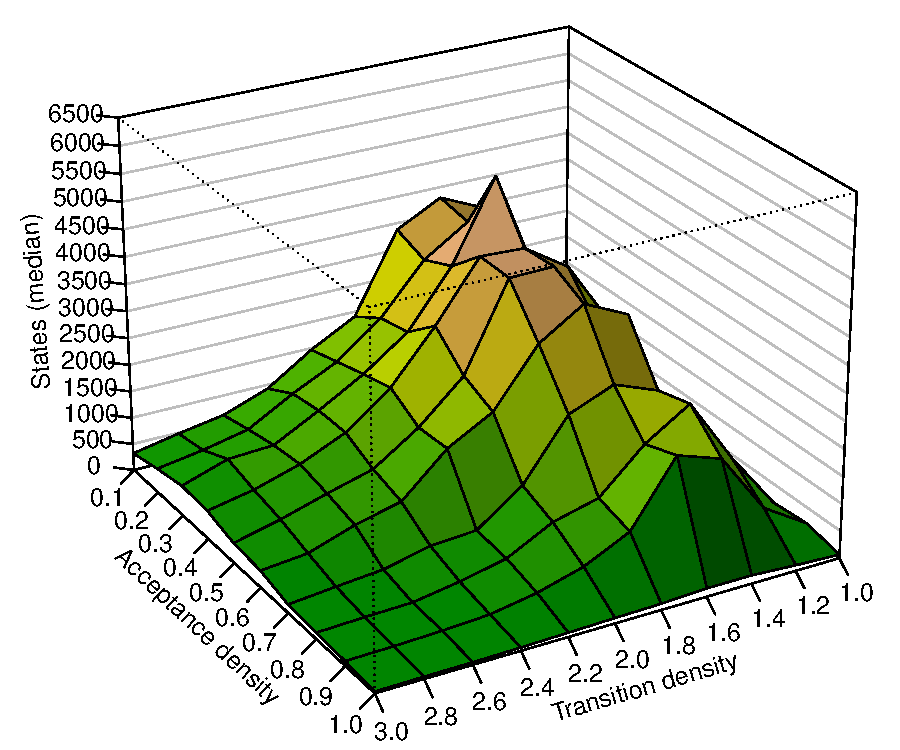
\includegraphics[width=\textwidth]{figures/r/internal/goal/s.median.Fribourg.pdf}
  \caption{Fribourg}
  \end{subfigure}
  \hfill
  \begin{subfigure}[t]{\perspwidth\textwidth}
  \centering
  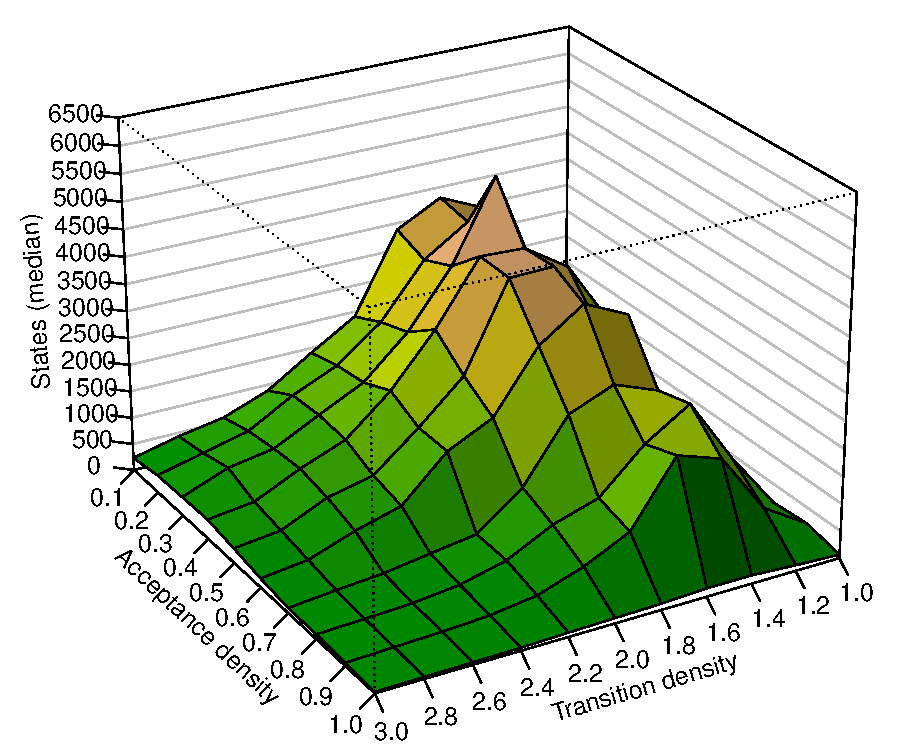
\includegraphics[width=\textwidth]{figures/r/internal/goal/s.median.Fribourg+R2C.pdf}
  \caption{Fribourg+R2C}
  \end{subfigure}
  \hfill

  \hfill
  \begin{subfigure}[t]{\perspwidth\textwidth}
  \centering
  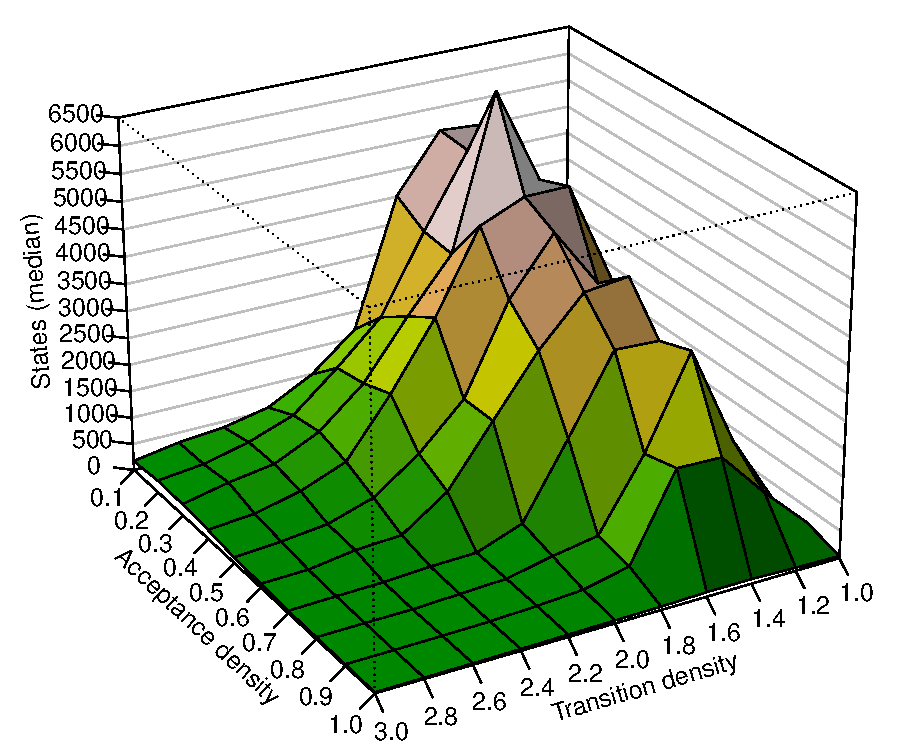
\includegraphics[width=\textwidth]{figures/r/internal/goal/s.median.Fribourg+R2C+C.pdf}
  \caption{Fribourg+R2C+C}
  \end{subfigure}
  \hfill
  \begin{subfigure}[t]{\perspwidth\textwidth}
  \centering
  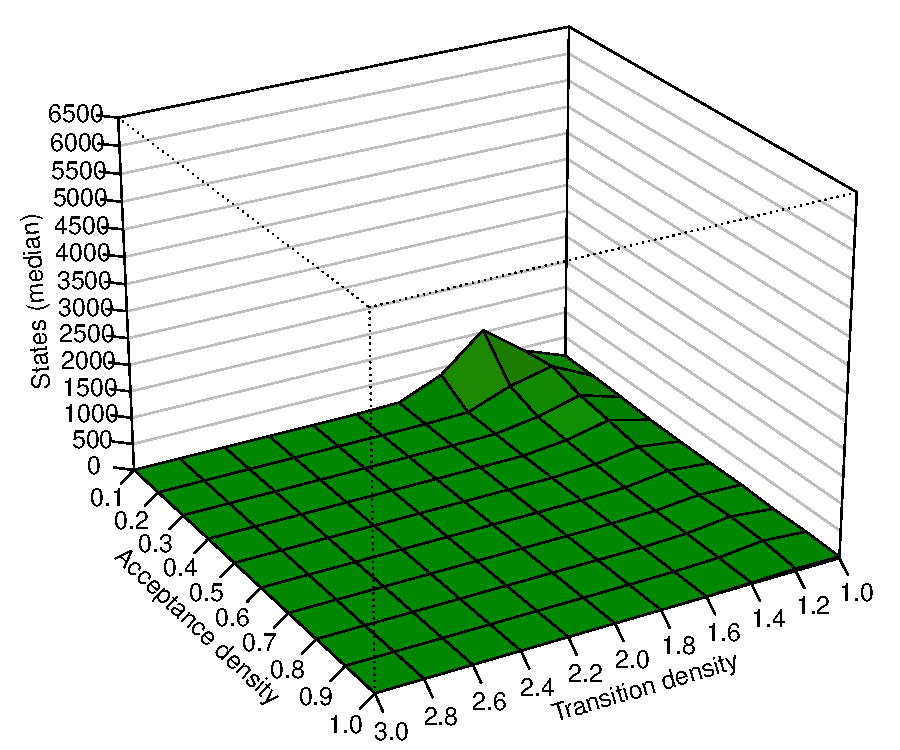
\includegraphics[width=\textwidth]{figures/r/internal/goal/s.median.Fribourg+R.pdf}
  \caption{Fribourg+R}
  \end{subfigure}
  \hfill  
\caption{Median complement sizes of the 10,939 effective samples of the internal tests for each of the 110 transition density/acceptance density classes of the \goal{} test set.}
\label{i.g.persp_1}
\end{figure}

As can be seen in the perspective plots of Figures~\ref{i.g.persp_1} and~\ref{i.g.persp_2}, there are large differences of the median complement sizes between the 110 transition density/acceptance density classes. All constructions exhibit a mountain (in some it is only a hill) roughly in the area between transition densities of 1.2 and 2.4, and acceptance densities of 0.1 and 0.9. The mountain is oblong, and its ridge runs across the entire spectrum of acceptance densities. The summit of the ridge is roughly at a transition density of 1.6. In the direction of lower acceptance densities, the mountain keeps its high altitude. In the direction of higher acceptance densities, on the other hand, the mountain gradually flattens down until nearly ground level at an acceptance density of 1.0.

Comparing the height of the mountains in the perspective plots with the overall median complement sizes in Table~\ref{i.g.stats} might be surprising at first. The mountains have a height of roughly 2,000--5,000 states (except Fribourg+R), which corresponds to the median complement sizes of the corresponding classes. On the other hand, the overall median complement size of all construction is 761 states or less. However, a closer look at the perspective plots (and the corresponding matrices in Appendix~\ref{app_matrices}) reveals that around half of the classes have a rather low median complement size ($< 1,000$) what justifies the low overall median complement sizes in Table~\ref{i.g.stats}. At the same time, this highlights the importance of a per-class analysis of the results on the \goal{} test set. It reveals much more accurately what to expect of the complementation of a specific automaton that resembles one of the classes of the \goal{} test set.

% Considering these median complement sizes in the perspective plots, apparently the automata of, for example, the class with a transition density of 1.6 and an acceptance density of 0.3 result in much larger complements than the automata of, for example, the class with a transition density of 3.0 and an acceptance density of 1.0. We could say that the automata of the first class are harder than the automata of the second class. Later in this section, we will try to identify hard, medium, and easy classes. For now, we will however focus on the relative differences between the different versions of the Fribourg construction.

Note that in the following, we will refer to specific points in the perspective plots as coordinates of the form $(t,a)$, where $t$ stands for the transition density, and $a$ for the acceptance density. For example, $(1.6,0.3)$ means the point at a transition density of 1.6 and an acceptance density of 0.3.

Let us now turn to the relative differences between the tested constructions. The plots of Fribourg and Fribourg+R2C in Figure~\ref{i.g.persp_1} (a) and (b) are rather similar. For both, the ridge has between 3,500 and 4,000 states with a peak of around 4,900 states at $(1.6, 0.3)$. In fact Fribourg+R2C only improves the performance on the complete input automata, compared to Fribourg. As we have analysed in Section~\ref{4_goal_testset}, the density of complete automata is highest in classes with high transition densities. By looking closely at the two plots, the values for the high transition density classes are indeed slightly lower for Fribourg+R2C than for Fribourg. Obviously, for classes that do not contain any complete automata, the values of the two constructions are identical.

Fribourg+R2C+C in Figure~\ref{i.g.persp_1} (c) has the highest mountain of all constructions. Its ridge has approximately 5,000 states, and it has a peak at $(1.6,0.3)$ of more than 6,000 states. This means basically that with Fribourg+R2C+C the ``mountain classes'' (the classes that result in large complements), result in even larger complements than for the other constructions. This might be surprising again, because as can be seen in Table~\ref{i.g.stats}, Fribourg+R2C+C has one of the lowest \textit{overall} median complement sizes. However, by comparing the classes with low median complement sizes of Fribourg+R2C+C with the other constructions, we see that they are indeed often even lower. This means that while the ``mountain classes'' have exceptionally high median complement sizes, the ``flatland classes'' have exceptionally low ones. This supports our previous proposition that the R2C+C combination, which includes the adding of a sink state to incomplete automata (which constitute 91\% of the \goal{} test set), makes easy complementation tasks easier and hard ones harder.


% an even higher mountain than the Fribourg and Fribourg+R2C. The top of the ridge is at around 5,000 states and the peak at the class 1.6/3.0 has close to 6,500 states. As already in the stripchart in Figure~\ref{i.g.stripchart}, Fribourg+R2C+C seems much worse than Fribourg+R2C at a first glance. However, as we have seen in Table~\ref{i.g.stats}, the median of Fribourg+R2C+C is 34.5\% lower than the median of Fribourg+R2C (689 to 451). By taking a closer look at the perspective plots of Fribourg+R2C and Fribourg+R2C+C, the reason for this can be seen. The low areas of Fribourg+R2C+C are slightly lower than the low areas of Fribourg+R2C. This is apparently enough to decrease the overall median. The much higher mountain peaks of Fribourg+R2C+C, on the other hand, do not influence the median. However, they show their effect in the overall mean which for Fribourg+R2C+C is 24\% higher than for Fribourg+R2C (2,424.6 to 1,955.9).

Fribourg+R in Figure~\ref{i.g.persp_1} (d) has, as expected, extremely low values for all the classes. In particular, 68 of the 110 classes have a median complement size of 1 (see corresponding matrix in Figure~\ref{i.g.matrices} (d) in Appendix~\ref{app_matrices}). We already hinted previously at the relation of a median complement size of 1 and the universal automata in the \goal{} test set. The per-class results of Fribourg+R reveal that all the classes with a median complement size of 1 contain 50 or more universal automata (compare matrices in Figure~\ref{i.g.matrices} (d) in Appendix~\ref{app_matrices} and Figure~\ref{testset_analysis} (b)). If all these universal automata are reduced by the R option to a single-state automaton, then it explains the observed median complement size of 1 for these classes (remember that there are 100 automata in each class). However, also the classes which contain less than 50 universal automata have significantly lower complement median sizes than in the Fribourg construction without the R option. This indicates that the Fribourg construction also  generates numerous unreachable and dead states for non-universal automata. 

% Comparing the fourth plot in Figure~\ref{i.g.persp_1}, Fribourg+R, to the plots of Fribourg, Fribourg+R2C, and Fribourg+R2C+C is like comparing a Dutch polder to the Swiss Alps. The mountain shrinks to a small hillock and the rest of the terrain is low and flat. This is because so many complements of the Fribourg construction can be reduced to very small sizes by removing their unreachable and dead states. The corresponding matrix in Appendix~\ref{app_matrices} reveals that 68 of the 110 classes have a median complement size of 1. If we further compare this matrix to the matrix with the number of universal automata in Figure~\ref{testset_analysis} (b) in Section~\ref{4_goal_testset}, we see that all the classes with a median of 1 contain more than 50 universal automata, and the classes with a median greater than 1 contain less than 50 universal automata. There is a total of 100 automata per class. This makes sense as the complements of universal automata are empty automata, and every empty automaton can be reduced to an automaton with a single non-accepting state. Looking at the classes with a median greater than 1, we see that their values are still considerably lower than the ones of the plain Fribourg construction.

\begin{figure}[ht]
\centering
  \hfill
  \begin{subfigure}[t]{\perspwidth\textwidth}
  \centering
  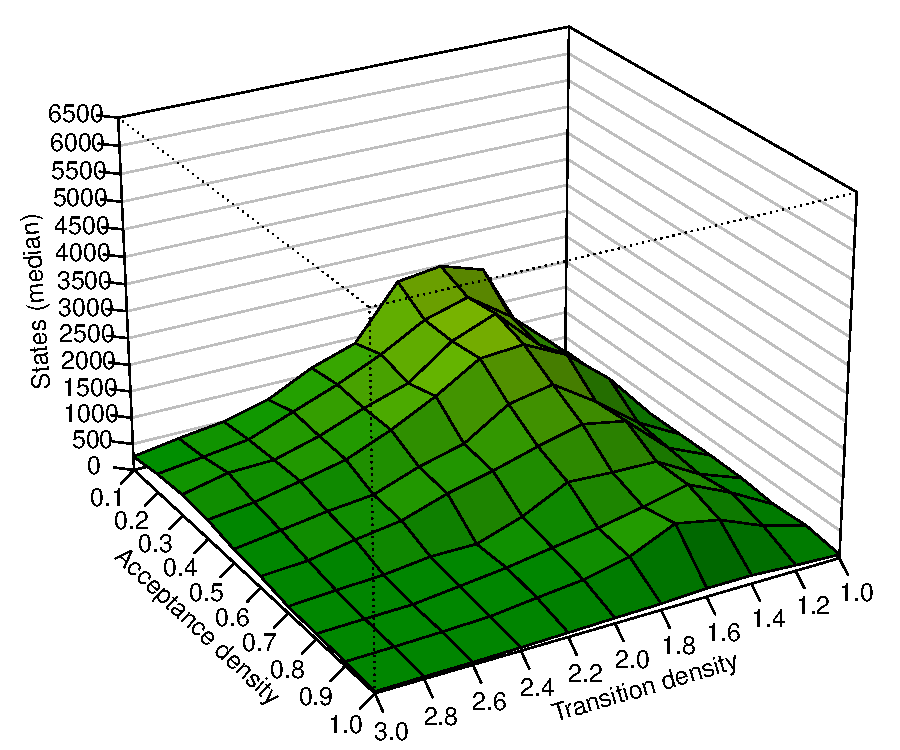
\includegraphics[width=\textwidth]{figures/r/internal/goal/s.median.Fribourg+M1.pdf}
  \caption{Fribourg+M1}
  \end{subfigure}
  \hfill
  \begin{subfigure}[t]{\perspwidth\textwidth}
  \centering
  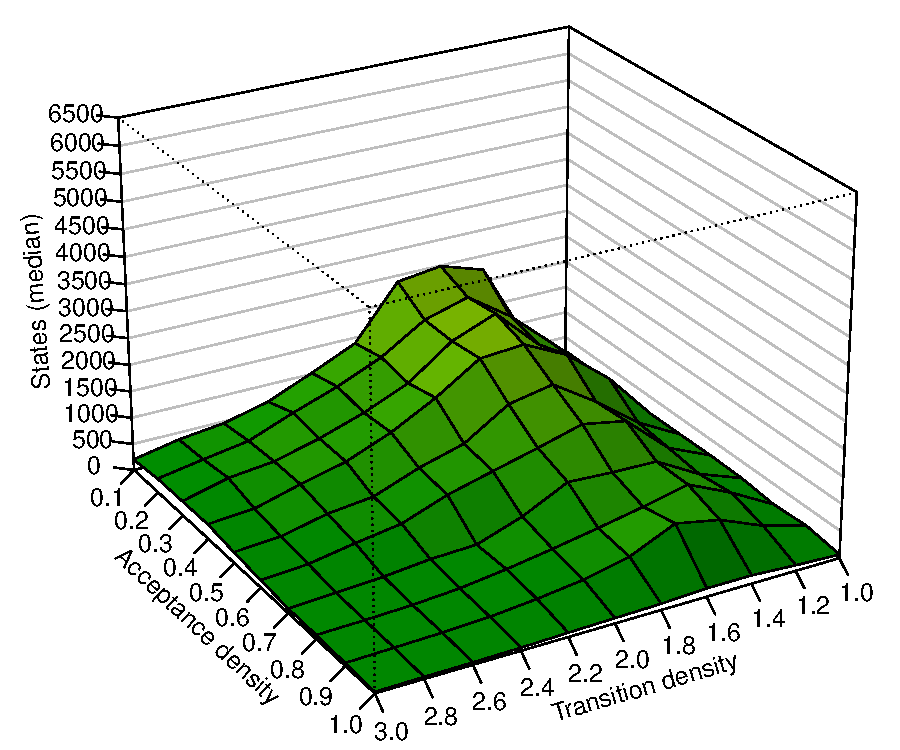
\includegraphics[width=\textwidth]{figures/r/internal/goal/s.median.Fribourg+M1+R2C.pdf}
  \caption{Fribourg+M1+R2C}
  \end{subfigure}
  \hfill

  \hfill
  \begin{subfigure}[t]{\perspwidth\textwidth}
  \centering
  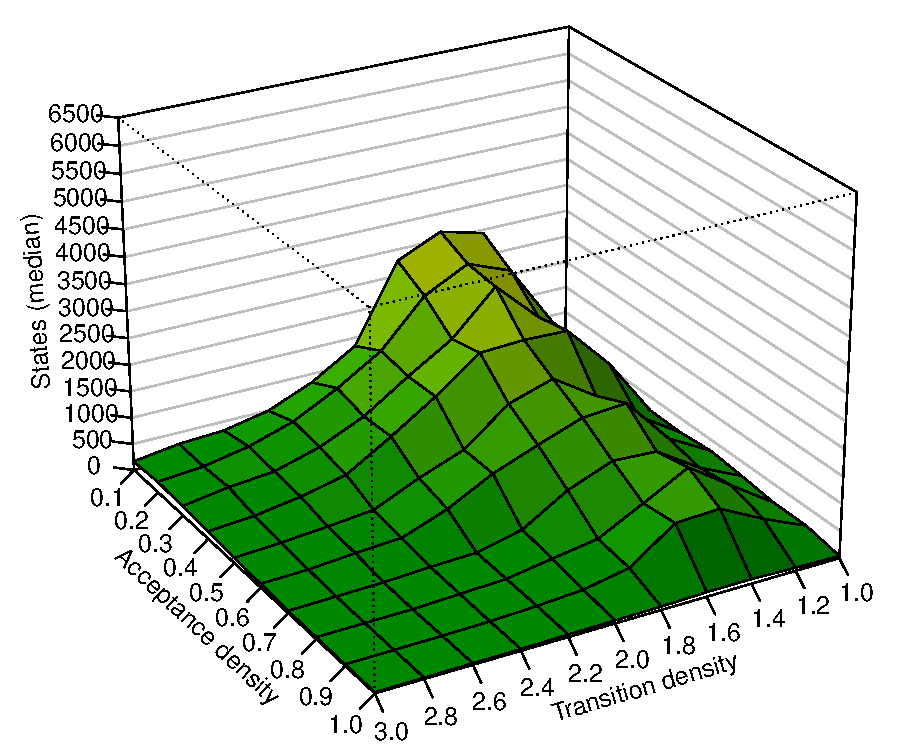
\includegraphics[width=\textwidth]{figures/r/internal/goal/s.median.Fribourg+M1+R2C+C.pdf}
  \caption{Fribourg+M1+R2C+C}
  \end{subfigure}
  \hfill
  \begin{subfigure}[t]{\perspwidth\textwidth}
  \centering
  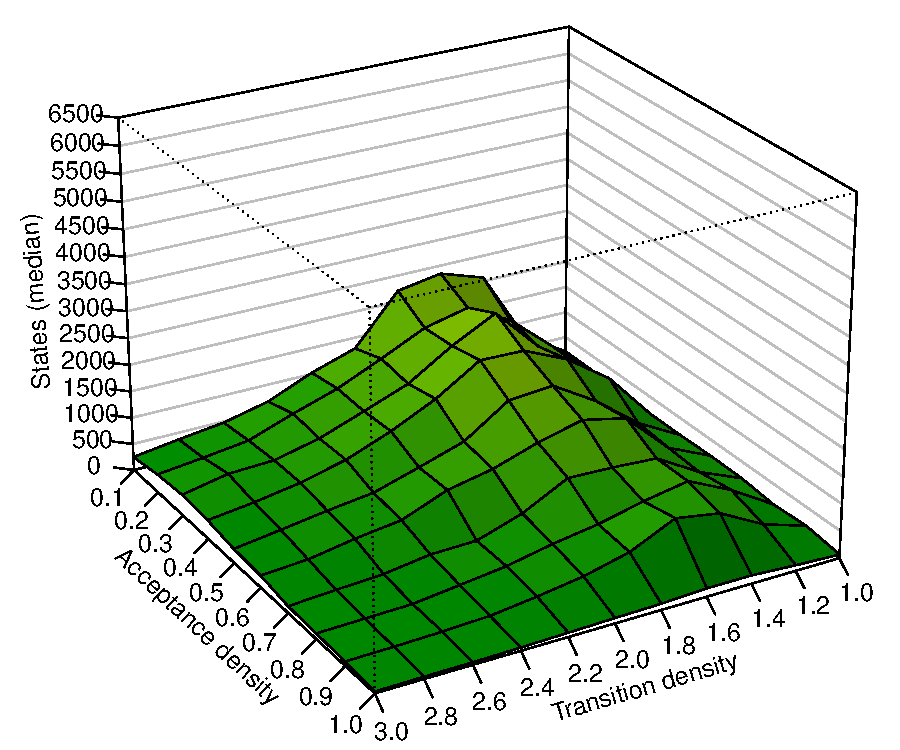
\includegraphics[width=\textwidth]{figures/r/internal/goal/s.median.Fribourg+M1+M2.pdf}
  \caption{Fribourg+M1+M2}
  \end{subfigure}
  \hfill
\caption{Median complement sizes of the 10,939 effective samples for each of the 110 transition density/acceptance density classes of the \goal{} test set.}
\label{i.g.persp_2}
\end{figure}

Figure~\ref{i.g.persp_2} shows the perspective plots for Fribourg+M1, Fribourg+M1+R2C, Fribourg+M1+R2C+C, and Fribourg+M1+M2. All of these versions include the M1 optimisation. The first three versions, Fribourg+M1, Fribourg+M1+R2C, and Fribourg+M1+R2C+C can be seen as pairs to Fribourg, Fribourg+R2C, and Fribourg+R2C+C, that additionally include the M1 optimisation. Most apparent by comparing these three pairs is that for the versions including M1 the mountain is significantly flatter. For Fribourg+M1 and Fribourg+M1+R2C the ridge has less than 2,500 states, as opposed to around 3,500 states for Fribourg and Fribourg+R2C. For Fribourg+M1+R2C+C the top of the ridge has around 3,000 states, as opposed to 5,000 states for Fribourg+R2C+C. This shows that the M1 optimisation causes a significant improvement for the automata of the ``mountain classes'', that is, the automata that generally result in larger complements. However, the M1 optimisation also has a positive effect on the automata of the ``flatland classes'', that is, the automata that typically result in smaller complements. This can be best seen in the corresponding matrices in Appendix~\ref{app_matrices}, or by comparing the overall means and  medians of the corresponding constructions with and without the M1 optimisation (see Table~\ref{i.g.stats}).

The relative differences between Fribourg+M1, Fribourg+M1+R2C, Fribourg+M1+R2C+C are very similar to the relative differences between Fribourg, Fribourg+R2C, and Fribourg+R2C+C. Also the reasons for these differences are basically the same, and caused by the R2C and C options, as we have previously explained for Figure~\ref{i.g.persp_1}.

Regarding Fribourg+M1+M2 in Figure~\ref{i.g.persp_2} (d), it is most interesting to compare it to Fribourg+M1, in order to isolate the effect of the M2 optimisation. From Table~\ref{i.g.stats}, we know that the overall median of Fribourg+M1+M2 is higher than the one of Fribourg+M1 (496 against 482), and the overall mean of Fribourg+M1+M2 is lower than the one of Fribourg+M1 (958.0 against 963.2). Comparing the per-class medians in the perspective plots of the two constructions does not reveal any salient differences, except that the highest values of Fribourg+M1+M2 seem to be slightly lower than the ones of Fribourg+M1. However, comparing the matrices of the two constructions in Figure~\ref{i.g.matrices} (e) and (h) reveals that Fribourg+M1+M2 has lower median complement sizes for almost all classes with acceptance densities between 0.1 and 0.4. On the other hand, Fribourg+M1+M2 has higher median complement sizes for most classes with an acceptance density between 0.5 and 0.9. Thus, the M2 optimisation indeed has a positive effect on the performance, but only on \textit{some} automata. These automata are those that contain not too many accepting states. On the other hand, for automata with 50\% or more accepting states, the M2 optimisation decreases the performance, rather than increasing it. For many complementation constructions, automata with few accepting states are harder to complement than automata with a lot of accepting states ~\cite{2011_tsai}. This means that the M2 optimisation is especially suitable for these automata that are hard for other constructions. This makes it interesting to apply this optimisation selectively on automata on which a positive effect is expected.

 % of the remaining four versions of the Fribourg construction, all of which include the M1 optimisation. Most apparent in these plots is that the mountain that we described for the plots of Fribourg, Fribourg+R2C, and Fribourg+R2C+C is still there, but it is rather a hill than a mountain. For Fribourg+M1, and Fribourg+M1+R2C, the height of the ridge is around 2,500 states. This is reflected by the overall means of these two versions compared to their counterparts without the M1 optimisation, Fribourg, and Fribourg+R2C. The decrease of the overall mean from Fribourg to Fribourg+M1 is by 52\% (from 2004.6 to 963.2) and from Fribourg+R2C to Fribourg+M1+R2C by 52.1\% (from 1955.9 to 937.7). The decreases of the overall medians are by 36.6\% (from 761 to 482), and 35.1\% (from 689 to 447) for the same two pairs of versions. With this we can confirm that the M1 optimisation brings a significant performance gain for the automata in the \goal{} test set.

% Regarding the M2 optimisation, we can see that the mountain ridge in the Fribourg+M1+M2 perspective plot is slightly lower than the one in the Fribourg+M1 perspective plot. The flatland regions, however, seem to not change much. This is reflected by the overall mean of Fribourg+M1+M2 which is slightly lower than in Fribourg+M1 (958.9 opposed to 963.2). The overall median, on the other hand, is higher for Fribourg+M1+M2 than for Fribourg+M1 (496 opposed to 482). An interpretation of this behaviour is that the application of the M2 optimisation results in smaller complements for \textit{some} input automata. \textcolor{red}{Better analysis: Fribourg+M1+M2 is better for almost all classes with an acceptance density up to 0.4, and worse for most of the classes with a n acceptance density between 0.5 and 0.9. The results are exactly identical for all the classes with an acceptance density of 1.0!}. \textcolor{gray}{These automata are especially the hard ones that produce large complements. This positive effect of M2 does however not affect enough input automata, especially not the easy automata, as to improve the overall performance of the construction in terms of the median complement sizes. As already stated previously, we consider therefore Fribourg+M1 as the better construction on the \goal{} test set than Fribourg+M1+M2.}

% Finally,Fribourg+M1+R2C+C differs from Fribourg+M1+R2C in a similar way that Fribourg+R2C+C differs from Fribourg+R2C. The higher regions get higher and the lower regions get lower, that is, a performance decline on hard automata, but a performance gain on easy automata. The performance gain on the easy automata is however effective enough to decrease the overall median from 447 to 331, which is minus 26\%.

% With 331 states, Fribourg+M1+R2C+C has the lowest median of all the versions (apart from the special case Fribourg+R). However, we still declare Fribourg+M1+R2C as the winner on the \goal{} test set, mainly for two reasons. First, while Fribourg+M1+R2C+C has a lower median, the mean is still higher (1062.6 to 937.7 which is a plus of 13.3\%). This results from the complements of the hard automata, which are larger than with Fribourg+M1+R2C. From a practical point of view, the mean might be relevant, because it relates more directly to the required computing resources than the median. Indeed, the execution per complementation task in CPU time is 25.4\% higher for Fribourg+M1+R2C+C than for Fribourg+M1+R2C (all measured execution time in CPU time are presented in Appendix~\ref{app_times}). The increase in the average execution time per automaton is from 4.44 to 5.57 seconds and in the total execution time from 48,572 seconds ($\approx$ 135 hours) to 60,919 seconds ($\approx$ 169 hours). Fribourg+M1+R2C, on the other hand, has the lowest mean of all versions. The second reason that we choose Fribourg+M1+R2C as the winner and not Fribourg+M1+R2C+C is that the C option is not a real part of the construction. It actually modifies the input automata before the construction starts in order to make them better suited for the construction. Fribourg+M1+R2C, on the other hand, includes only construction-specific options.

\subsubsection{Difficulty Categories}
The per-class analysis shows that there are big difference in the complement sizes across the transition density/acceptance density classes of the \goal{} test set. Furthermore, there is a certain pattern throughout the results of all construction, namely the mountain and the flatland regions. In the following, we attempt to categorise the classes of the \goal{} test set into \textit{easy}, \textit{medium}, and \textit{hard} categories. 

To this end, we calculated for each transition density/acceptance density class the average of the median complement sizes of all the tested constructions. This results in a matrix containing the average median complement sizes for each class. Then, we defined two breakpoints at 500 and at 1,600 states that divide the classes into easy, medium, and hard ones. The result of this analysis is shown in Figure~\ref{i.g.difficulty}.

\begin{figure}[ht]
\centering
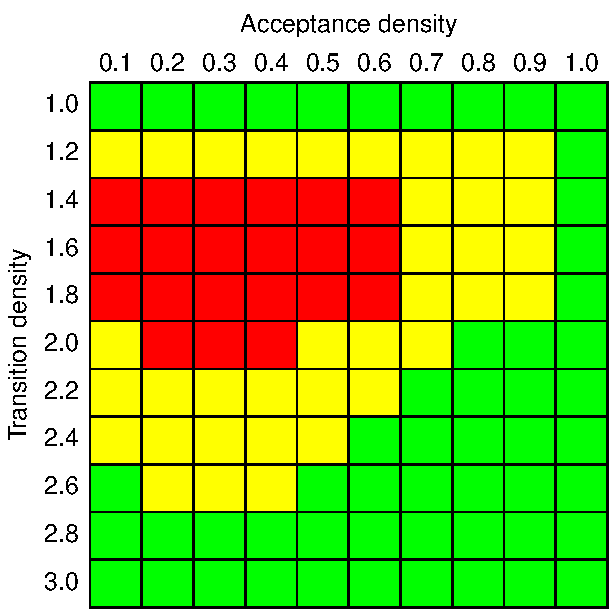
\includegraphics[width=0.35\textwidth]{figures/r/internal/goal/difficulty.pdf}
\caption{Difficulty categories \textit{easy} (green), \textit{medium} (yellow), and \textit{hard} (red) of the 110 transition density/acceptance density classes of the \goal{} test set.}
\label{i.g.difficulty}
\end{figure}

Figure~\ref{i.g.difficulty}, shows a total of  53 easy, 36 medium, and 21 hard classes. The easy classes are mainly those with extreme values. All the classes with a transition density of 0.1, or 2.8 and 3.0, and a high acceptance density of 1.0 are easy. Furthermore, there is a ``triangle'' of easy classes between transition densities 2.0 and 2.6. and acceptance densities 0.5 and 0.9. The lower the transition density, the higher the acceptance density must be such that the class is classified as easy. The hard classes are roughly those with a transition density between 1.4 and 1.8 and an acceptance density between 0.1 and 0.6. The medium classes finally are located as a ``belt'' around the hard classes.

It is interesting to see that the hard automata are those with a ``medium'' transition density between 1.4 and 1.8. This range of transition densities means that every state has on average 1.4 to 1.8 outgoing transitions for each symbol of the alphabet. Somehow this specific level of connectivity seems to make the complementation of an automaton very hard. If the connectivity is lower, complementation becomes easier, and if the connectivity is harder, complementation becomes easier as well. A reason that complementation becomes easier with a lower transition density might be that such automata may contain unreachable and disconnected state. We let further investigations on the influence of the transition density on the complementation difficulty for future work.

Figure~\ref{i.g.difficulty} also shows that automata with a larger number of accepting states are generally easier to complement. This proposition has been made by Tsai et al.~\cite{2011_tsai}, and it is the base of the MACC option (maximising acceptance set) of many complementation construction in \goal{} (see Section~\ref{4_goal}). Summarising, we can say that a transition density between 1.4 and 1.8 makes automata hard to complement, but that this difficulty is alleviated by an increasing acceptance density.

Note that these results are specific to the Fribourg construction, and cannot be readily generalised to other complementation constructions. Furthermore the results are based exclusively on the \goal{} test set with its specific types of automata. However, as we will see in the results of the external tests in Section~\ref{5_external_goal}, other complementation constructions show a similar behaviour on the automata of the \goal{} test set.

% It is interesting that the extreme values of transition and acceptance densities result in easy automata. With a transition density of 1.0 and an alphabet size of 2, each of the 15 states has on average two outgoing and two incoming transitions. With a transition density of 3.0, each state has on average 6 outgoing and 6 incoming transitions. These low or high connectivity seems to considerably simplify the complementation task. The same applies to a high acceptance density of 1.0, which means that every state is an accepting state.

% Generally, we can say that automata with high acceptance densities are easier to complement than automata with lower acceptance densities. This also means that the pattern of easy automata at the extreme values of transition and acceptance density, does not apply to to the lower extreme of the acceptance density. Automata with a very low acceptance density of 0.1 are hard to complement---unless they are made easy by a low or high transition density.

% Another interesting point is that the hard automata have transition densities between 1.4 and 1.8. It seems that this range of transition densities is the crucial factor in the hardness of a complementation task, and that it is only alleviated by a growing acceptance density. This explains the decline of the mountain ridge from low to high acceptance density values.

% Summarising we can say that transition densities between 1.4 and 1.8 produce the hardest complementation tasks, and that to the both sides the difficulty steadily decreases with declining or growing transition density. Furthermore, a growing acceptance density generally implies easier complementation tasks.


\subsection{Michel Test Set}
\label{5_internal_michel}
The Michel test set consists of the four Michel automata Michel~1, Michel~2, Michel~3, and Michel~4 as pictured in Figure~\ref{michel_automata} of Chapter~\ref{chap_investigation}. These automata have of 3, 4, 5, and 6 states, and an alphabet size of 2, 3, 4, and 5, respectively. The versions of the Fribourg construction that we tested on the Michel test set are the following (see Section~\ref{4_internal}):

\begin{enumerate}
\item Fribourg
\item Fribourg+R2C
\item Fribourg+M1
\item Fribourg+M1+M2
\item Fribourg+M1+M2+R2C
\item Fribourg+R
\end{enumerate}

Below, we first present the complement sizes of the Michel automata resulting from the different versions. Next, we discuss the corresponding state growths (number of states of the complement relative to the number of states of the input automaton) and bring them in relation with the worst-case state growths. Finally, we present the measured execution times for the individual complementation tasks. 

\subsubsection{Complement Sizes}
In Table~\ref{i.m.states}, we present the resulting complement sizes for all versions and all the Michel automata. The column \textit{Fitted~curve} contains a function of the form $(an)^n$. This function was obtained by fitting a curve of this form to the four $xy$-points of each construction, with the $x$-values being the sizes of the input automata, and the $y$-values the sizes of the corresponding complements. The used fitting method is the method of non-linear least squares. The column \textit{Std.~error} shows the standard error that results from the fit.

\begin{table}[htb]
\centering
% latex table generated in R 3.1.2 by xtable 1.7-4 package
% Sun Aug 16 00:19:45 2015
\begin{tabular}{lrrrrrr}
  \hline
Construction & Michel 1 & Michel 2 & Michel 3 & Michel 4 & Fitted curve & Std. error \\ 
  \hline
Fribourg & 57 & 843 & 14,535 & 287,907 & $(1.35n)^n$ & 0.01\% \\ 
  Fribourg+R2C & 33 & 467 & 8,271 & 168,291 & $(1.24n)^n$ & 0.06\% \\ 
  Fribourg+M1 & 44 & 448 & 5,506 & 81,765 & $(1.10n)^n$ & 0.07\% \\ 
  Fribourg+M1+M2 & 42 & 402 & 4,404 & 57,116 & $(1.03n)^n$ & 0.12\% \\ 
  Fribourg+M1+M2+R2C & 28 & 269 & 3,168 & 43,957 & $(0.99n)^n$ & 0.04\% \\ 
  Fribourg+R & 18 & 95 & 528 & 3,315 & $(0.64n)^n$ & 0.35\% \\ 
   \hline
\end{tabular}

\caption{Complement sizes for the Michel automata 1 to 4, having 3 to 6 states.}
\label{i.m.states}
\end{table}

% In the second-last column ``Fitted curve'' of Table~\ref{i.m.states}, we fitted a function of the form $(an)^n$ to the measured four data points. These data points consist of the sizes of the four Michel automata (3, 4, 5, and 6) as the $x$-values ad the corresponding complement sizes as the $y$-values. The fitted function $(an)^n$ can be seen as an ``averaged'' state growth of these four automata ($n$ is the size of the input automaton). The last column ``Std. error'' contains the standard error that resulted from the fit.

The first four column of Table~\ref{i.m.states} reveal the massive state growth that the Michel automata provoke. This can be best seen in the results of Michel~4. This automaton has 6 states and an alphabet size of 5. The first tested version, Fribourg, complements Michel~4 to an automaton with 287,907 states. This is a much higher state growth than we observed for any of the automata in the \goal{} test set. Note that the maximum complement size of Fribourg for the \goal{} test set is 37,904 (see Table~\ref{i.g.stats}). However, the \goal{} automata have 15 states, and Michel~4 has just 6 states, which makes a big difference with an exponential state growth. At the end of this section, we extrapolate complement sizes of Michel automata with 7 and more states, by assuming the state growth observed for the Michel automata up to 6 states.

Fribourg+R2C complements Michel~4 to an automaton with 168,291 states (note that Michel automata are complete, and thus the R2C optimisation has an effect). Compared to the result of Fribourg, this is a reduction of 41.5\%. This means that 41.5\% of the states produced by Fribourg have a rightmost component with colour 2, which can be removed.

The M1 optimisation of Fribourg+M1 has an even more positive effect than the R2C optimisation. The complement produced by Fribourg+M1 has 81,765 states, which is 71.6\% less than the complement of Fribourg. This indicates that the M1 optimisation is particularly efficient for hard automata.

Fribourg+M1+M2 complements Michel~4 to an automaton with only 57,116 states. This is smaller than the complement of Fribourg+M1, and the same applies to the other Michel automata. This is interesting, because for the \goal{} test set,  from an overall point of view, Fribourg+M1+M2 is less efficient than Fribourg+M1 (see Table~\ref{i.g.stats}). However, as we analysed for the individual transition density/acceptance density of the \goal{} test set, Fribourg+M1+M2 is actually more efficient than Fribourg+M1 for a certain type of automata. These automata are the ones with an acceptance density up to 0.4. The four tested Michel automata all have an acceptance density of 0.33 or less, and thus fall in this category. Hence, the fact that Fribourg+M1+M2 is more efficient on the Michel automata than Fribourg+M1 coincides with this observation for the \goal{} test set.

Fribourg+M1+M2+R2C further decreases the complement size of Michel~4 to 43,957. Again, this is because the R2C optimisation removes all the states whose rightmost component has colour 2. Compared to Fribourg, the complement produced by Fribourg+M1+M2+R2C is 84.7\% smaller. In other words, the application of all the three optimisations to the Fribourg construction, cuts the complement size of Michel~4 in approximately six and a half.

Finally, the complement size of Fribourg+R for Michel~4 is 3,315. This means that 284,592, or 98.8\%, of the states produced by Fribourg are unreachable or dead states, that are removed by the R option.

\subsubsection{State Growth Functions}
The heavy state growth of Michel automata make them suitable to be used as lower bounds for the worst-case state complexities of the tested constructions, in case these worst-case complexities have not yet been determined precisely. To this end, we calculated for each construction a state growth function in the second-last column of Table~\ref{i.m.states}.

For Fribourg, the state growth of the Michel automata is $(1.35n)^n$, whereas the determined upper bound for the worst-case is $O((1.59n)^n)$ (see Section~\ref{3_lower_part}). This means that whatever the actual worst-case state growth of Fribourg is, it cannot be lower than $(1.35n)^n$, because with our empirically determined complement sizes of the Michel automata, we have a proof that Fribourg can generate $(1.35n)^n$ many states, with $n$ being the number of states of the input automaton.

Regarding the other versions, for Fribourg+R2C this lower bound is $(1.24n)^n$. However, for Fribourg+R2C, we do not have a theoretically calculated upper bound of the worst-case state complexity. For Fribourg+M1, the state growth of the Michel automata is $(1.10n)^n$, whereas the calculated worst-case state growth is $O((1.195n)^n)$\footnote{This is actually the worst-case state growth of the lower part of the automaton. For the overall worst-case state growth, the maximum number of states of the upper part of $(0.53n)^n$ must be added to it. However, the resulting term is clearly dominated by $O((1.195n)^n)$.}. This means that for Fribourg+M1, the gap between the upper and lower bound is relatively small, and the worst-case state growth cannot be further improved very much.

For Fribourg+M1+M2, the state growth of the Michel automata is $(1.03n)^n$. However, the worst-case state growth has been calculated to be $O((0.86n)^n)$, even with evidence that it might actually be $O((0.76n)^n)$. So, here we seem to have a discrepancy. Whereas we have the empirical proof that Fribourg+M1+M2 can produce $(1.03n)^n$ many states, with $n$ being the number of states of the input automaton, the theoretically calculated results state that Fribourg+M1+M2 can generate at most $O((0.86n)^n)$ or $O((0.76n)^n)$ many states. The reason for this discrepancy might be hidden in the big-$O$ notation. The functions $O((0.86n)^n)$ or $O((0.76n)^n)$ are not exact, but rather the result of omitting constant factors and lower order terms. We leave further investigations on this point for future work.

For the last two versions, Fribourg+M1+M2+R2C and Fribourg+R, the measured state growths are $(0.99n)^n$ and $(0.64n)^n$, respectively. However, for these versions we do not have theoretically calculated upper bounds for the worst-case state complexity.

\subsubsection{Execution Times}
In Table~\ref{i.m.times}, we present the execution times of the different versions for complementing the Michel automata. The reported values are in in CPU time seconds. As mentioned, the measurement of execution times is dependent on many factors, such as the implementation and the execution environment, and thus should be interpreted with care. However, for the case of the Michel automata, we think that the execution times still provide interesting insights.

\begin{table}[htb]
\centering
% latex table generated in R 3.1.2 by xtable 1.7-4 package
% Sun Aug 16 16:21:25 2015
\begin{tabular}{lrrrrrr}
  \hline
Construction & Michel 1 & Michel 2 & Michel 3 & Michel 4 & Fitted curve & Std. error \\ 
  \hline
Piterman+EQ+RO & 2.5 & 3.8 & 42.6 & 75,917.4 & $(1.08n)^n$ & 0.64\% \\ 
  Slice+P+RO+MADJ+EG & 2.3 & 3.6 & 11.4 & 159.5 & $(0.39n)^n$ & 0.38\% \\ 
  Rank+TR+RO & 2.2 & 3.0 & 6.4 & 30.0 & $(0.29n)^n$ & 0.18\% \\ 
  Fribourg+M1+M2+R2C & 2.5 & 3.5 & 10.8 & 2,332.6 & $(0.61n)^n$ & 0.62\% \\ 
   \hline
\end{tabular}

\caption{Execution times for the Michel automata 1 to 4, having 3 to 6 states.}
\label{i.m.times}
\end{table}

For Michel~1, all versions take slightly more than 2 seconds. Approximately 2 seconds are actually caused by the start-up of the Java Virtual Machine, which is also included in our time measurements. For Michel~2, all versions take 4 seconds or less, and for Michel~3 all versions are still under 1.5 minutes. For Michel~4, however, the execution times seem to explode. Fribourg takes 100,976.0 seconds, which are approximately 28 hours. However, this time is considerably lower Fribourg+R2C, which takes 27,938.3 seconds, or 7.76 hours. Fribourg+M1 takes 6,508.4 seconds, or 1.8 hours. The best version, Fribourg+M1+M2+R2C, takes 2,332.6 seconds, or 39 minutes. Note that Fribourg+R takes the same time as Fribourg, plus an additional delay to remove the unreachable and dead states.

There are two remarkable points in these execution times. First, the increase of the execution times between Michel~3 and Michel~4 is much bigger than the increase of the complement sizes between Michel~3 and Michel~4. For example, for Fribourg, the complement size of Michel~4 is about 20 times bigger than the complement size of Michel~3. However, the execution time for Michel~4 is approximately 1,138 times bigger than execution time for Michel~3. As another example, for Fribourg+M1+M2+R2C the factors are 14 for the complement size and 216 for the execution time. Second, the differences of the execution times between the different versions are larger than the corresponding differences between the complement sizes. For example, for Michel~4, the complement of Fribourg+M1+M2+R2C is around 6.5 times smaller than the complement of Fribourg. However the execution time of Fribourg+M1+M2+R2C is 43 times smaller than the execution time of Fribourg. In summary, this shows that with an increasing number of states the required computation time increases disproportionately.


\subsubsection{Extrapolations}
As promised, below we extrapolate the complement sizes and execution times for larger Michel automata. To this end, we fitted functions of the form $(an)^n$ to the measured execution times in Table~\ref{i.m.times} in the same way as we did for the complement sizes. The parameter $n$ is the number of states of the input automaton, and the value of the functions is the required execution time of the complementation task in CPU time seconds. Based on the fitted functions for Fribourg, we present in Table~\ref{i.m.extrapolation} the extrapolated values for the Michel automata~5 to~8.


% The fitted functions that we calculated for the measured complement sizes and execution times are based on only four data points. This is generally not enough to make reliable extrapolations. However, it is still interesting to do such an extrapolation in order to see the involved complexity and to show why we were restricted to include only the first four Michel automata in the test set. In Table~\ref{i.m.extrapolation}, we show extrapolated values for the complement sizes and execution times for the plain Fribourg construction (the least efficient one), based on the corresponding fitted functions. The table includes the extrapolated values for the Michel automata 5 to 8, which have 7 to 10 states. 

\begin{table}[htb]
\centering
\begin{tabular}{lrrrr}
\hline
Automaton & States ($n$) & Compl. size $(1.35n)^n$ & Exec. time $(1.14n)^n$ & $\approx$ days/months/years \\
\hline
Michel 5 &  7 &       6,882,980 &      2,020,385 &     23 days   \\
Michel 6 &  8 &     189,905,394 &     46,789,245 &     18 months \\
Michel 7 &  9 &   5,939,189,262 &  1,228,250,634 &     39 years  \\
Michel 8 & 10 & 207,621,228,081 & 36,039,825,529 &  1,142 years  \\
\hline
\end{tabular}
\caption{Extrapolated complement sizes and execution times for the Michel automata~5 to~8 based on the fitted growth function of Fribourg.}
\label{i.m.extrapolation}
\end{table}

As can be seen, the complementation of Michel~5 would take 23 days with Fribourg. This is still a conservative estimation, because, as we have seen, the execution time grows disproportionately fast with an increasing number of states. A duration of 23 days would already exceed the maximum running time of a job on the cluster we use for our experiments. This shows why we restricted ourselves to include only the Michel automata~1 to~4 in the Michel test set. And even if Michel~5 would still be doable, the execution times of 18 months, 39 years, and 1,142 years for Michel~6, 7, and~8, are most probably too long for an empirical study, even for a master's thesis.

% According to the fitted state growth function, the complement of Michel~5 would have nearly 7 million states, and the complement of Michel~8 even more than 207 billion states. Already the computation of the 7 million states of Michel~5 would most probably exceed the available memory resources in our computing environment. Regarding execution time, the complementation of Michel~5 would take 23 days. This would by far exceed the maximal running time of a job on our computer cluster. And even if we would not have these administrative time restriction, the time to wait for the complementation of Michel~5 to~8, between 18 months and 1,142 years, is definitely too long, even for a master's thesis.




% The special version Fribourg+R yields very small complements compared to the other versions. This tells us that the complements of the other versions contain a large number of unreachable and dead states. For example, the complement of Michel~4 of Fribourg+R (3,315 states) is 1.2\% of the size of the complement of Fribourg. This means that 98.8\% of the 287,907 states of the complement of Fribourg are unreachable and dead states. This is actually not surprising, because, following the proof of Michel~\cite{michel1988}\cite{1996_thomas}, the smallest possible complement of Michel~4 has 24 states. This is because Michel~4 has $m=4$ and Michel proved that the complement has at least size $m!$. This means that that even after reducing all the unreachable and dead states from the complement of Fribourg, an even much smaller complement would still be possible.

% Up to now we just looked at the specific results of Michel~4. The fitted functions of the form $(an)^n$ summarise the results of all the four Michel automata. These functions give us reference points for the worst-case state complexities of the different versions of the Fribourg construction. For example, for the plain Fribourg construction with its fitted function of $(1.35n)^n$, we have now the proof that this construction produces complements of size $(1.35n)^n$, where $n$ is the size of the input automaton. This means that the worst-case complexity cannot be lower than $(1.35n)^n$ (but it can still be higher). This bound decreases for the different versions of the Fribourg construction down to $(0.99n)^n$ for Fribourg+M1+M2+R2C.

% In Table~\ref{i.m.times} we show the measured execution time in seconds (CPU time) for each complementation task. We can see that the difference between the least and most efficient version is bigger than for the complement sizes. For example for Michel~4, Fribourg+M1+M2+R2C is more than 43 times faster than Fribourg (2,332.6 seconds compared to 100,976 seconds). In more familiar unities, this corresponds to approximately 39 minutes for Fribourg+M1+M2+R2C against 28 hours for Fribourg. We also fitted functions of the form $(an)^n$ to the measured execution times where $n$ is the number of states of the input automaton, and the value of the function is the execution time of the task in CPU time seconds.





\section{Results of the External Tests}
\label{5_external}
The external tests consist of the comparison of the best version of the Fribourg construction on each test set against three other complementation constructions. These three other constructions are the following (see Section~\ref{4_external}):

\begin{itemize}
\item Piterman+EQ+RO
\item Slice+P+RO+MADJ+EG
\item Rank+TR+RO
\end{itemize}

Regarding the versions of the Fribourg construction, we declared the best we declared the best one on each test set to be the following:

\begin{itemize}
\item Fribourg+M1+R2C    \tabto{4.2cm} for the \goal{} test set
\item Fribourg+M1+M2+R2C \tabto{4.2cm} for the Michel test set
\end{itemize}

In the subsequent two sections, we first present the results of these tests on the \goal{} test set (Section~\ref{5_external_goal}), followed by the results on the Michel test set (Section~\ref{5_external_michel}).


\subsection{GOAL Test Set}
\label{5_external_goal}
In this section, we analyse the results of the external tests on the \goal{} test set in a similar way as we did for the internal tests. That is, we determine the effective samples, analyse the complement sizes from an overall point of view, and on a per-class basis for each of the 110 transition density/acceptance density of the \goal{} test set.

However, there is an issue that caused us to slightly modify our scheme of analysis. One of the constructions, Rank, exhibits an exceptionally bad performance on the \goal{} test set compared to the other constructions. The result is that the set of effective samples is reduced by more than one third. By using this reduced set of effective samples, we exclude a big part of the results of the other three constructions, Piterman, Slice, and Fribourg. To prevent this from influencing the interpretation of the results of these constructions, we present two separate analyses, one with Rank, and one without Rank. In the following, we first discuss the effective samples (with and without Rank), and then present the two versions of the result analysis with and without Rank. 


\subsubsection{Effective Samples}
Table~\ref{e.g.outs} shows the number of timeouts and memory excesses for all four tested construction. Like for the internal tests, the timeout is set to 600 seconds CPU time, and the memory limit to 1 GB Java heap size. As can be seen, there is a very high number of excesses for Rank. The construction timed out for 3,713 automata, and exceeded the memory for 83 automata. This gives a total of 3,796, or 34.5\%, of aborted complementation task. This contrasts with the other constructions. There are only two timeouts for Piterman, and one for Fribourg.

\begin{table}[ht]
\centering
% latex table generated in R 3.1.2 by xtable 1.7-4 package
% Sat Jun  6 16:42:17 2015
\begin{tabular}{lrr}
  \hline
Construction & Timeouts & Memory excesses \\ 
  \hline
Fribourg & 48 & 0 \\ 
  Fribourg+R2C & 30 & 0 \\ 
  Fribourg+R2C+C & 54 & 0 \\ 
  Fribourg+M1 & 2 & 0 \\ 
  Fribourg+M1+M2 & 1 & 0 \\ 
  Fribourg+M1+R2C & 1 & 0 \\ 
  Fribourg+M1+R2C+C & 8 & 0 \\ 
  Fribourg+R & 48 & 0 \\ 
   \hline
\end{tabular}

\caption{Number of timeouts and memory excesses of the external tests on the \goal{} test set.}
\label{e.g.outs}
\end{table}

By including all four constructions, there are 7,204 effective samples, which are 65.5\% of the test set. On the other hand, by including only Piterman, Slice, and Fribourg, there are 10,998 effective samples. This means that by including Rank, we exclude more than one third of the results of Piterman, Slice, and Fribourg that are actually available. As mentioned, for this reason, in the following, we present two separate analyses, one for the 7,204 effective samples with Rank, and another one for the 10,998 effective samples without Rank.

\subsubsection{With Rank}
Figure~\ref{e.g.stripchart.with_rank} shows a stripchart with the complement sizes of the 7,204 effective samples. As can be seen, Rank has a very long tail with a maximum reaching 120,000 states. This stripchart makes apparent that there is a very high number of automata for which Rank produces much larger complements than the other constructions. Regarding the other constructions, Piterman has clearly the highest density of small complements, whereas Slice and Fribourg have similar distribution.

\begin{figure}[htb]
\centering
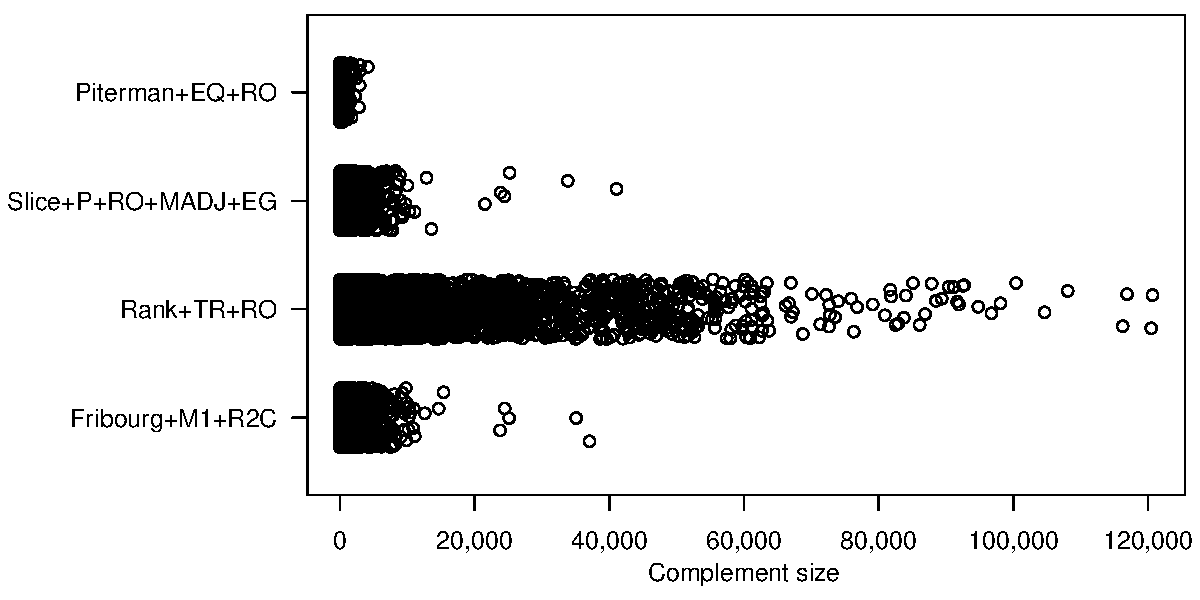
\includegraphics[scale=0.575]{figures/r/external/goal/s.stripchart.with_rank.pdf}
\caption{Complement sizes of the 7,204 effective samples of the external tests \textit{with Rank} on the \goal{} test set.}
\label{e.g.stripchart.with_rank}
\end{figure}

In Table~\ref{e.g.stats.with_rank}, we present the mean and the five-number summary of the complement sizes of the 7,204 effective samples. Regarding Rank, this table bears a surprise. The 25th percentile and the median of Rank are comparable to the other constructions, and even lower than for the Fribourg construction. However, this picture changes dramatically for the 75th percentile, which seems to explode compared to the other constructions. This means that, despite the bad image that Rank conveys in the stripchart and by the mean complement size, for at least half of the 7,204 effective samples, Rank performs perfectly comparable to the other constructions. Only for at most the other half of these automata, Rank performs poorly and results in very large complements. This is a remarkable fact, and it would be an interesting task for future work to investigate which characteristics cause an automaton to be hard for Rank.

\begin{table}[htb]
\centering
% latex table generated in R 3.1.2 by xtable 1.7-4 package
% Sun Aug 16 15:57:19 2015
\begin{tabular}{lrrrrrr}
  \hline
Construction & Mean & Min. & P25 & Median & P75 & Max. \\ 
  \hline
Piterman+EQ+RO & 106.0 & 1 & 29.0 & 58.0 & 121.0 & 4,126 \\ 
  Slice+P+RO+MADJ+EG & 555.4 & 2 & 70.0 & 202.0 & 596.0 & 41,081 \\ 
  Rank+TR+RO & 5,255.6 & 2 & 81.0 & 254.5 & 3,178.2 & 120,674 \\ 
  Fribourg+M1+R2C & 662.9 & 2 & 101.0 & 269.0 & 754.5 & 37,068 \\ 
   \hline
\end{tabular}

\caption{Statistics of the complement sizes of the 7,204 effective samples of the external tests \textit{with Rank} on the \goal{} test set.}
\label{e.g.stats.with_rank}
\end{table}

Regarding the other constructions in Table~\ref{e.g.stripchart.with_rank}, again Piterman is the clear winner. Slice and Fribourg have comparable results, although the values are in the favour of Slice.

We omit the analysis of the complement sizes for each of the transition density/acceptance density classes, because the low number of effective samples causes many classes to be not represented at all in the effective samples. Instead, in the following, we pass over directly to the second version of the analysis which excludes Rank.

% And indeed, the 25th percentile and the median of Rank are higher than for Piterman and Slice, but still lower than for our Fribourg construction. This means that the Rank construction produces more smaller complements than the Fribourg construction. However, the picture changes dramatically for the 75th percentile where the value of Rank is more than four times higher than the value for Fribourg. Also the mean of Rank is many times higher than the means of all the other constructions. A possible explanation for this is that the Rank construction has a comparable performance with the other constructions for easy automata. For harder automata, however, the performance of Rank is much worse than the other constructions. In addition, the automata that are hardest for Rank are not even included in this analysis as it includes only the 7,204 effective samples. The 3,796 automata that are excluded would probably have resulted in even larger complements with the Rank construction.

% What we cannot tell is whether the automata which are hard for Rank are the same that are hard for the other constructions. However, as we will see later, we think that this is not necessarily the case.

\subsubsection{Without Rank}
Considering only Piterman, Slice, and Fribourg, there are 10,998 effective samples. Figure~\ref{e.g.stripchart} shows a stripchart with the complement sizes of these 10,998 automata for each construction. The stripchart presents a similar picture as we already saw in the previous analysis with the Rank construction. Piterman clearly has the highest density of small complements, whereas Slice and Fribourg have comparable distributions.

% Given the large number of aborted complementation tasks of Rank we decided to do the main analysis and comparison of the results without the Rank construction. Because with the Rank construction would basically exclude more than one third of the tasks that have been successfully completed by the other constructions from the result analysis. Our main interest is however to compare the performance of the Fribourg construction to the other constructions. In this way, we would probably miss important aspects in the result analysis of the other three constructions. 

% Without the Rank construction there are 10,998 effective samples In Figure~\ref{e.g.stripchart} we display the complement sizes of these 10,998 effective samples as a stripchart.

\begin{figure}[ht]
\centering
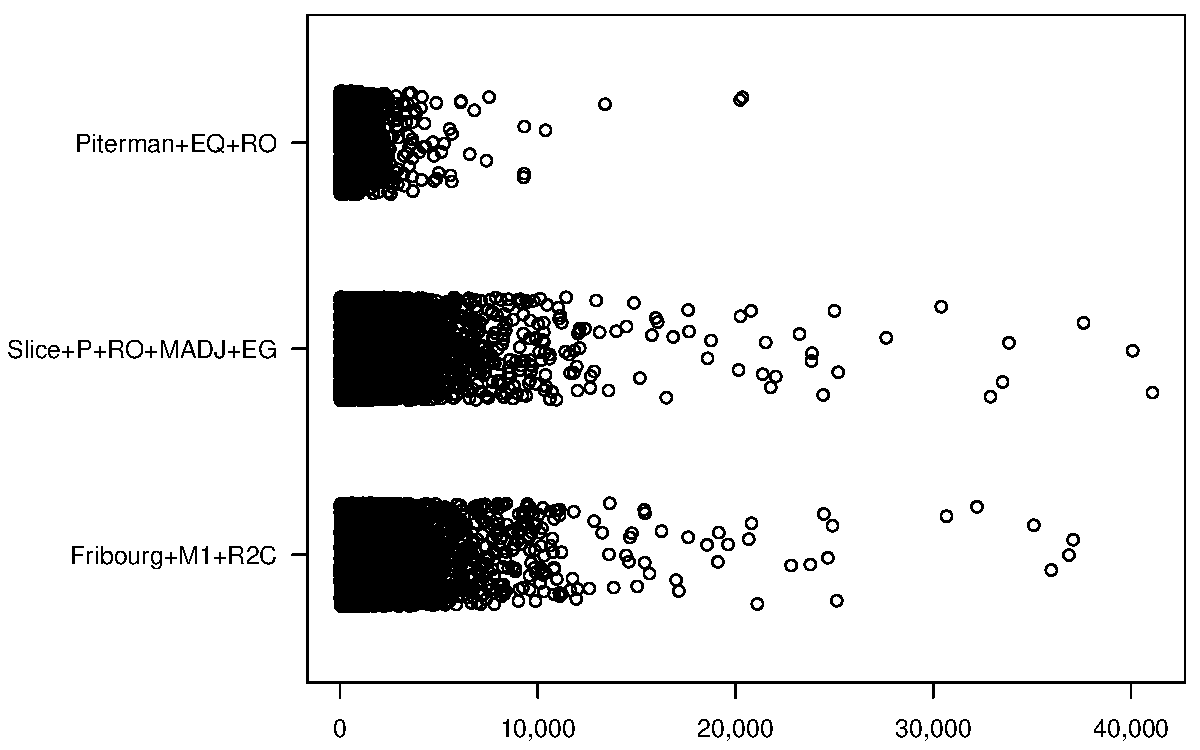
\includegraphics[scale=0.575]{figures/r/external/goal/s.stripchart.pdf}
\caption{Complement sizes of the 10,998 effective samples of the external tests \textit{without Rank} on the \goal{} test set.}
\label{e.g.stripchart}
\end{figure}

In Table~\ref{e.g.stats}, we present the mean and the five-number summary of the complement sizes of these constructions. These numbers confirm that Piterman is by far the most performant construction on the \goal{} test set. Its values for mean, median, 25th and 75th percentile are multiple times lower than the values of the other two constructions.  Regarding Slice and Fribourg, Slice has the better results than Fribourg. The mean, 25th percentile, median, and 75th percentile of Slice are 6.7\%, 21.6\%, 12.4\%, and 11.6\%, respectively, lower than for Fribourg. These results allow to rank the three constructions according to their overall performance on the \goal{} test set. First is, by a large margin, Piterman, second is Slice, and third is Fribourg.

\begin{table}[ht]
\centering
% latex table generated in R 3.1.2 by xtable 1.7-4 package
% Sat Jun  6 16:42:20 2015
\begin{tabular}{lrrrrrr}
  \hline
Construction & Mean & Min. & P25 & Median & P75 & Max. \\ 
  \hline
Piterman+EQ+RO & 209.6 & 1 & 38.0 & 80.0 & 183.0 & 20,349 \\ 
  Slice+P+RO+MADJ+EG & 949.4 & 2 & 120.0 & 396.0 & 1,003.0 & 41,081 \\ 
  Fribourg+M1+R2C & 1,017.3 & 2 & 153.0 & 452.0 & 1,134.0 & 37,068 \\ 
   \hline
\end{tabular}

\caption{Statistics of the complement sizes of the 10,998 effective samples of the external tests \textit{without Rank} on the \goal{} test set.}
\label{e.g.stats}
\end{table}

Next, we analyse the complement sizes for each of the 110 transition density/acceptance density classes of the \goal{} test set. Like for the internal tests, we consider the median complement size for each class. Figure~\ref{e.g.persp} shows the perspective plots for Piterman, Slice, and Fribourg. Note that we provide the corresponding matrices with the exact values in Appendix~\ref{app_matrices} (Figure~\ref{e.g.matrices}). Also note that the perspective plot of Fribourg+M1+R2C in Figure~\ref{e.g.persp} (c) is the same as the one we presented for the internal tests in Figure~\ref{i.g.persp_2} (c), however, with a different $z$-axis scale.

\renewcommand{\perspwidth}{0.3}
\begin{figure}[ht]
\centering
  \hfill
  \begin{subfigure}[t]{\perspwidth\textwidth}
  \centering
  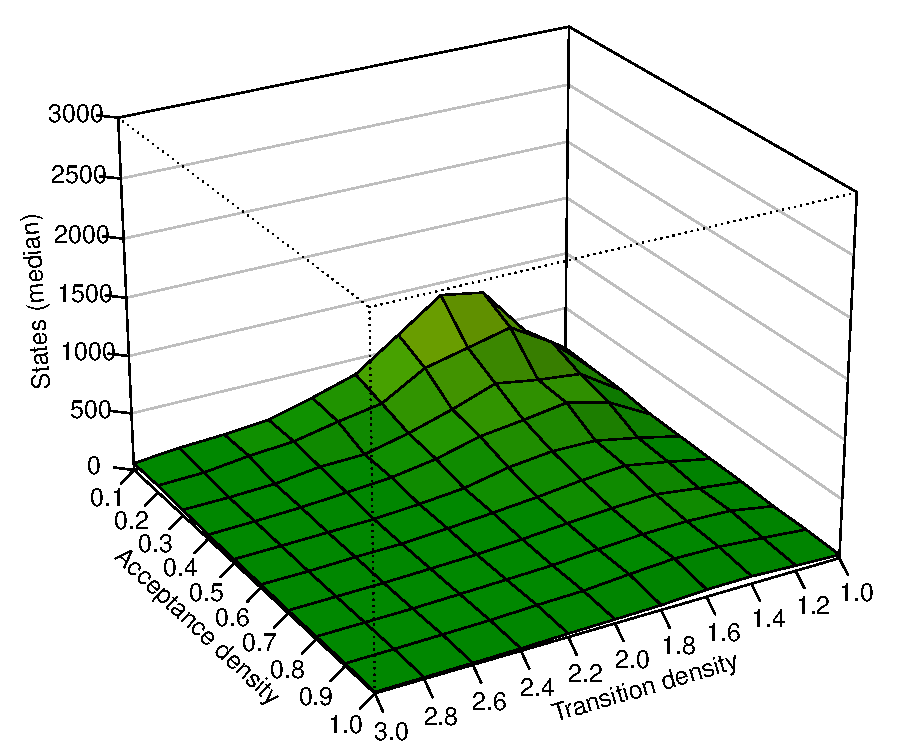
\includegraphics[width=\textwidth]{figures/r/external/goal/s.median.Piterman+EQ+RO.pdf}
  \caption{Piterman+EQ+RO}
  \end{subfigure}
  \hfill
  \begin{subfigure}[t]{\perspwidth\textwidth}
  \centering
  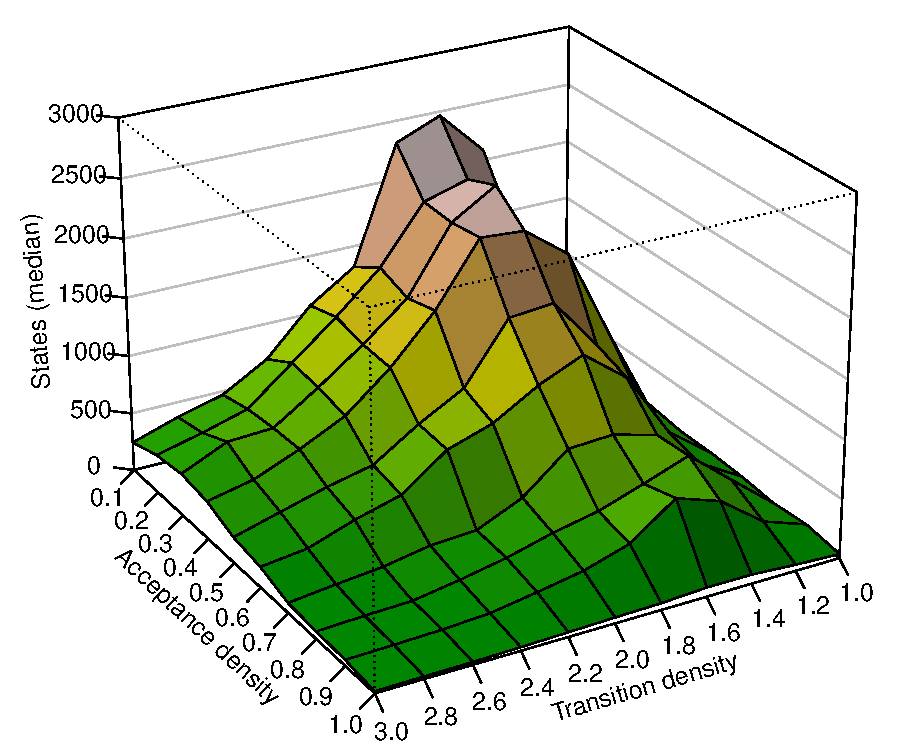
\includegraphics[width=\textwidth]{figures/r/external/goal/s.median.Slice+P+RO+MADJ+EG.pdf}
  \caption{Slice+P+RO+MADJ+EG}
  \end{subfigure}
  \hfill
  \begin{subfigure}[t]{\perspwidth\textwidth}
  \centering
  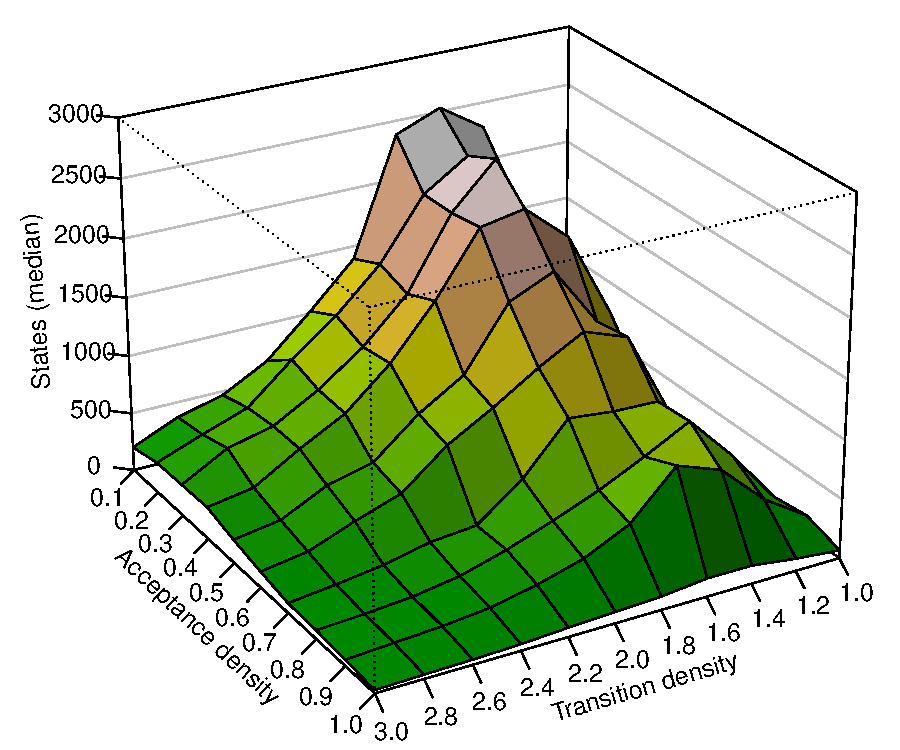
\includegraphics[width=\textwidth]{figures/r/external/goal/s.median.Fribourg+M1+R2C.pdf}
  \caption{Fribourg+M1+R2C}
  \end{subfigure}
  \hfill
\caption{Median complement sizes of the 10,998 effective samples of the external tests \textit{without Rank} for each of the 110 transition density/acceptance density classes of the \goal{} test set.}
\label{e.g.persp}
\end{figure}

The perspective plots reveal for Piterman a significantly lower median complement size throughout all classes. It seems as if Piterman is more performant by a constant factor for all types of automata. However, the basic pattern, namely the mountain around a transition density of 1.6 and low acceptance densities, is the same for Piterman as for the other two constructions, merely in a reduced form. Regarding Slice and Fribourg, the two constructions exhibit a very similar pattern. A small difference is that Fribourg has slightly worse values for classes with a transition density up to 2.0, but often slightly better values for classes with a higher transition density. This means that, roughly, Fribourg performs slightly worse than Slice on the hard automata and slightly better on many easy automata.

The similar patterns of the different constructions in Figure~\ref{e.g.persp} show that the classification into easy, medium, and hard automata of the \goal{} test set, that we established for the Fribourg construction (see Section~\ref{5_internal_goal}), is also applicable to other complementation constructions. At least for Piterman and Slice, the same automata seem to be hard and easy as for the Fribourg construction.

% In the perspective plots we can see that the pattern for Fribourg and Slice are very similar. The median complement sizes in the individual classes do not differ a lot, both relatively and absolutely. However, the medians of Fribourg seem to be throughout (with some exceptions) slightly higher than the ones of Slice. This means that Fribourg and Slice seem to have similar strengths and weaknesses, but Slice is slightly more efficient on the tested automata.

% Piterman, as expected, has medians that are multiple times lower than the corresponding medians of Fribourg and Slice. The basic pattern, however, is still similar. There is a mountain ridge along the classes with a transition density of 1.6 with its top in the class with transition density 1.6 and acceptance density 0.1.


\subsection{Michel Test Set}
\label{5_external_michel}
For the Michel test set, we compare Fribourg+M1+M2+R2C against the same three versions of Piterman, Slice, and Rank as for the external tests on the \goal{} test set. 

\subsubsection{Complement Sizes}
Table~\ref{e.m.states} shows the complement sizes of the Michel automata~1 to~4 for each of the tested constructions. Like for the internal tests, we fitted a function of the form $(an)^n$ to the measured complement sizes, and provide the standard error resulting from the fit in the last column.

\begin{figure}[htb]
\centering
% latex table generated in R 3.1.2 by xtable 1.7-4 package
% Sun Aug 16 00:19:45 2015
\begin{tabular}{lrrrrrr}
  \hline
Construction & Michel 1 & Michel 2 & Michel 3 & Michel 4 & Fitted curve & Std. error \\ 
  \hline
Fribourg & 57 & 843 & 14,535 & 287,907 & $(1.35n)^n$ & 0.01\% \\ 
  Fribourg+R2C & 33 & 467 & 8,271 & 168,291 & $(1.24n)^n$ & 0.06\% \\ 
  Fribourg+M1 & 44 & 448 & 5,506 & 81,765 & $(1.10n)^n$ & 0.07\% \\ 
  Fribourg+M1+M2 & 42 & 402 & 4,404 & 57,116 & $(1.03n)^n$ & 0.12\% \\ 
  Fribourg+M1+M2+R2C & 28 & 269 & 3,168 & 43,957 & $(0.99n)^n$ & 0.04\% \\ 
  Fribourg+R & 18 & 95 & 528 & 3,315 & $(0.64n)^n$ & 0.35\% \\ 
   \hline
\end{tabular}

\caption{Complement sizes for the Michel automata 1 to 4, with 3, 4, 5, and 6 states, respectively.}
\label{e.m.states}
\end{figure}

The values in Table~\ref{e.m.states} contain a series of surprising results. First, Rank produces the smallest complements for all Michel automata. Note that this is the same Rank construction which performs exceptionally bad on the \goal{} test set, and which therefore we had to exclude from the result analysis of the \goal{} test set. For the Michel automata, however, Rank beats all the other constructions by a large margin.

The next surprise is that Piterman has the worst result for Michel~4. Again, this is the same Piterman construction that has by far the best performance on the \goal{} test set. However, note that the bad performance of Piterman applies particularly to Michel~4. For Michel~3, Piterman has only the second-worst result, for Michel~2, it has the second-best, and for Michel~1, it has even the best result (together with Rank). It would be interesting to test how the performance of Piterman evolves with Michel~5 and beyond. However, as we have demonstrated in Section~\ref{5_internal_michel}, for practical reasons this is nearly impossible.

Another surprise is that Fribourg performs relatively well on the Michel automata. For Michel~3, Fribourg is ranked second behind the unbeatable Rank with a large gap to the third-placed construction (Piterman). For Michel~4, Fribourg is also ranked second behind Rank, but with an even much larger gap to the third-placed construction (Slice). In particular, the complement of Fribourg for Michel~4 is 2.8 times smaller than the complement of Slice, and 4 times smaller than the complement of Piterman.

In summary, if we take the fitted curves (or the results on Michel~4) as the overall measure, then the ranking of the four construction is, first Rank, second Fribourg, third Slice, and fourth Piterman. Note that this is the reverse ranking of the same constructions on the \goal{} test set, where the best is Piterman, second Slice, third Fribourg, and fourth Rank (however, the version of the Fribourg construction used for the \goal{} test set is Fribourg+M1+R2C instead of Fribourg+M1+M2+R2C). This shows that it is generally not possible to declare a certain construction to be ``better'' than another in a universal sense. A construction can only be better than another with respect to a certain automaton, or set of automata.

\subsubsection{Execution Times}
As for the internal tests, we also present the execution times of the external tests on the Michel automata. Table~\ref{e.m.times} shows the measured execution times in CPU time seconds. The second-last column of the table again contains a growth function of the form $(an)^n$ that we fitted to the the input automaton sizes and corresponding execution times. The last column of the table contains the standard error of the fit.

\begin{table}[htb]
\centering
% latex table generated in R 3.1.2 by xtable 1.7-4 package
% Sun Aug 16 16:21:25 2015
\begin{tabular}{lrrrrrr}
  \hline
Construction & Michel 1 & Michel 2 & Michel 3 & Michel 4 & Fitted curve & Std. error \\ 
  \hline
Piterman+EQ+RO & 2.5 & 3.8 & 42.6 & 75,917.4 & $(1.08n)^n$ & 0.64\% \\ 
  Slice+P+RO+MADJ+EG & 2.3 & 3.6 & 11.4 & 159.5 & $(0.39n)^n$ & 0.38\% \\ 
  Rank+TR+RO & 2.2 & 3.0 & 6.4 & 30.0 & $(0.29n)^n$ & 0.18\% \\ 
  Fribourg+M1+M2+R2C & 2.5 & 3.5 & 10.8 & 2,332.6 & $(0.61n)^n$ & 0.62\% \\ 
   \hline
\end{tabular}

\caption{Execution times for the Michel automata 1 to 4. These automata have 3, 4, 5, and 6 states, respectively.}
\label{e.m.times}
\end{table}

As can be seen in Table~\ref{e.m.times}, the execution times of all constructions stay relatively low until Michel~3. This is basically the same phenomenon that we observed for the internal tests on the Michel test set. But then, for Michel~4, the differences between the constructions are enormous. Rank takes just 30 seconds to complement Michel~4. On the other hand, Piterman takes 75,917.4 seconds, which are approximately 21 hours. Slice is  with 159.5 seconds also very fast. On the other hand Fribourg is with 2,332.6 seconds, or 39 minutes, significantly slower than Rank and Slice, but still much faster than Piterman.

From the results of the internal tests on the Michel test set, we learned that the execution time increases disproportionately with the number of generated states. This explains in parts the large time gap between Rank and Piterman for Michel~4. While Piterman's complement of Michel~4 is around 6.7 times larger than Rank's complement of Michel~4, Piterman's execution time is approximately 2,530 times longer than Rank's execution time. However, the extent of this disproportionate growing of the execution time is still surprising.

Another remarkable point is that Fribourg has a very long execution time for Michel~4 compared to Slice. This cannot be explained by the disproportionate growing of the execution time, because the complement produced by Fribourg is smaller than the complement produced by Slice. In detail, the complement of Fribourg is 2.8 times smaller than the complement of Slice, however, the execution time of Fribourg is 14.6 times greater than the execution time of Slice. There are two possible explanations for this. Either Slice is exceptionally fast on Michel~4, or Fribourg is exceptionally slow. To find this out, we would need to include further constructions in the test, which is a point that could be done in future work.

This concludes the presentation of the results of our empirical performance investigation of the Fribourg construction, consisting of the internal and external tests, on the \goal{} test set and the Michel test set. In the next section, we discuss important aspects of these results, and of the study in general.

% In Table~\ref{e.m.times} we present the execution times per complementation task in CPU time seconds. As for the complement sizes, we fitted a function of the form $(an)^n$ to the measured execution times where $n$ is the size of the input automaton.

% \begin{table}[ht]
% \centering
% % latex table generated in R 3.1.2 by xtable 1.7-4 package
% Sun Aug 16 16:21:25 2015
\begin{tabular}{lrrrrrr}
  \hline
Construction & Michel 1 & Michel 2 & Michel 3 & Michel 4 & Fitted curve & Std. error \\ 
  \hline
Piterman+EQ+RO & 2.5 & 3.8 & 42.6 & 75,917.4 & $(1.08n)^n$ & 0.64\% \\ 
  Slice+P+RO+MADJ+EG & 2.3 & 3.6 & 11.4 & 159.5 & $(0.39n)^n$ & 0.38\% \\ 
  Rank+TR+RO & 2.2 & 3.0 & 6.4 & 30.0 & $(0.29n)^n$ & 0.18\% \\ 
  Fribourg+M1+M2+R2C & 2.5 & 3.5 & 10.8 & 2,332.6 & $(0.61n)^n$ & 0.62\% \\ 
   \hline
\end{tabular}

% \caption{Execution times for the first four Michel automata.}
% \label{e.m.times}
% \end{table}

% Most interesting in Table~\ref{e.m.times} is the column with the times for Michel~4. The time difference between the best and the worst construction is enormous. While the Rank construction took just 30 seconds to complement Michel~4, the Piterman construction took 75,917.4 seconds which is approximately 21 hours. This is more than 2500 times longer. Of course the Piterman construction produced a bigger automata, which naturally requires more time, however, the automaton produced by the Piterman construction is just around 6.7 times bigger than the one of the Rank construction. This means that the Piterman construction must include very inefficient processes before finally arriving at the output automaton.

% Furthermore, we can see in Table~\ref{e.m.times} that also the Fribourg construction took relatively long to complement Michel~4 compared to Rank, namely 2,332.6 seconds which are approximately 39 minutes. This is 77.8 times longer than the 30 seconds of Rank. At the same time, Fribourg's complement has just 68.2\% more states than Rank's complement. Similarly, compared to the Slice construction the Fribourg construction is slow for Michel~4. Slice's complement is 2.8 times bigger than Fribourg's complement, but with 159.5 seconds the complementation of slice was 14.6 times faster than the complementation of Fribourg.

% So there seems to an inefficiency in the Fribourg construction in terms of execution time for the complementation of Michel~4. However, this inefficiency is by far not as pronounced as for Piterman. While the complement of Piterman is just 4 times bigger, the execution time of Piterman is 32.5 times longer than the one of the Fribourg construction. One could also look at it from the other side and say that not the Fribourg construction is inefficient on Michel~4, but that Rank and Slice are extremely efficient on this automaton.

% Finally, these interesting differences in the execution times between the four constructions can only be observed for Michel~4. For Michel~3 there are also differences but they are by far not as pronounced as for Michel~4. If the computational resources would allow it, it would be very interesting to run the constructions on Michel~5 and beyond. One thing that stays the same for all the four Michel automata is that Rank is always the fastest and Piterman always the slowest construction.

\section{Discussion}
\label{5_discussion}
In this section, we discuss the results that we presented in the previous section. This inludes a short summary of the most important results in Section~\ref{5_summary}. In Section~\ref{5_insights}, we describe the main insights into Büchi complementation in general that can be derived from our results. Finally, in Section~\ref{5_limitations}, we discuss the limitations of our study. 

\subsection{Summary of the Results}
\label{5_summary}
In the following, we recapitulate the most important results from earlier in this chapter. We first review the results related to the \goal{} test set, followed by the results related to the Michel test set.

\subsubsection{\goal{} Test Set}
Regarding the different versions of the Fribourg construction, we identified Fribourg+M1+R2C as the version with the best overall performance on the \goal{} test set. Interestingly, the application of the M1 and M2 optimisations together (Fribourg+M1+M2) results in a worse overall performance on the \goal{} test set than the application of the M1 optimisations alone (Fribourg+M1). However, we found out that this penalty introduced by Fribourg+M1+M2 does not apply to all automata types. Actually, Fribourg+M1+M2 has a better performance than Fribourg+M1 for all automata classes with an acceptance density between 0.1 and 0.4. However, for most other automata classes, Fribourg+M1+M2 performs indeed worse than Fribourg+M1, and this is enough to tilt the overall performance in the favour of Fribourg+M1. Another result is that the application of the R2C optimisation together with the C options results in many more large complements, but at the same time in many more small complements than the corresponding version without R2C and C. A way to see this is that R2C and C together make easy complementation tasks easier, an harder complementation tasks harder.

Regarding the other tested constructions, Piterman has a significantly better performance on the \goal{} test set than all the other constructions. This is true from an overall point of view and for each of the transition density/acceptance density classes of the \goal{} test set. The other extreme is Rank, which exhibits significantly worse performance on the \goal{} test set than all the other constructions. The best version of the Fribourg construction on the \goal{} test set (Fribourg+M1+R2C) and Slice have a comparable performance on the \goal{} test set, although there is a slight advantage for Slice.

We identified criteria that make the automata of the \goal{} test set result in larger or smaller complements, or in other words, make automata harder or easier to complement. For the Fribourg construction, the automata with a transition density between 1.4 and 1.8, and an acceptance density between 0.1 and 0.6 are the hardest complementation tasks. A higher or lower transition density makes the complementation of an automaton by trend easier. Furthermore, a higher acceptance density makes the complementation of an automaton by trend easier as well. Our results of Piterman and Slice suggest that these criteria also apply to other complementation constructions.

% Complement characteristics (overall)
% - Median couple of hundred states (below hundred only Piterman)
% - 75th percentile 1000-2000 states (by a large margin below 1000 only Piterman)
% - Maximum couple of 10,000 states

% Fribourg construction
% - Best version of Fribourg construction on goal test set: Fribourg+M1+R2C
% - Fribourg+M1 overall better on goal test set than Fribourg+M1+M2
% - Fribourg+M1+M2 better on automata with transition density up to 0.4 of goal test set than Fribourg+M1
% - Fribourg+R2C+C has more large complements but lower median complement size than other versions (makes easy automata easier and hard aut. harder)

% Other constructions
% - Piterman by far better than Fribourg and Slice on goal test set
% - Fribourg and Slice similar on goal test set (but Slice slightly better)
% - Rank very bad on goal test set

% Differences between classes
% - diverse complement sizes in goal test set
% - same pattern of complement sizes in goal test set for different constructions
% - Hard automata in goal test have transition density 1.4 - 1.8 and acceptance density up to 0.6 (for Fribourg)
% - Lower transiton density implies easier, and higher transition density implies easer (for Fribourg)
% - Higher acceptance density implies easier (for Fribourg)
% - Difficulty distribution is similar for other constructions (Piterman and Slice


\subsubsection{Michel Test Set}
We identified Fribourg+M1+M2+R2C as the best version of the Fribourg construction on the Michel test set. Interestingly, for the Michel automata, the application of the M1 and M2 optimisation together (Fribourg+M1+M2) results in a significantly better performance than the application of the M1 optimisation alone (Fribourg+M1). However, as we identified for the \goal{} test set, there are indeed certain types of automata for which Fribourg+M1+M2 performs better than Fribourg+M1. The Michel automata seem to belong to these type of automata. Generally, the R2C, M1, and M2 optimisations significantly increase the performance of the Fribourg construction on the Michel automata. Their simultaneous application (Fribourg+M1+M2+R2C) cuts the complement size of the largest Michel automata (Michel~4) by 6.5, and the execution time by 43.3, compared to the Fribourg construction without optimisations.

Regarding the other tested complementation constructions, Rank has by far the best performance on the Michel automata. This is one of the most surprising results, because Rank has by far the worst overall performance on the \goal{} test set. On the other hand, Piterman has by far the worst performance on the largest Michel automaton (Michel~4). This is again surprising, because Piterman has by far the best performance on all the automata types in the \goal{} test set. The best version of the Fribourg construction on the Michel test set (Fribourg+M1+M2+R2C) has the second-best overall performance on the Michel test set after Rank. The gap between Fribourg and the first-placed Rank is smaller than the gap between Fribourg and the third-placed Slice. However, the execution time of Fribourg for Michel~4 is significantly greater than the execution time of Rank and Slice. In general, Rank and Slice can be seen as extremely fast on the largest tested Michel automaton (Michel~4).


% Fribourg constrcution
% - Best version of Fribourg construction on michel test set: Fribourg+M1+M2+R2C
% - Fribourg+M1+M2 better on michel test set than Fribourg+M1

% Other constructions
% - Rank very good on Michel test set (best)
% - Piterman worst on Michel test set (Michel 4)
% - Fribourg second-best on michel test set
% - Friourg slow on Michel 4 compared to Slice and Rank, but fast compared to Piterman
% - Extreme differences in execution times on Michel 4 (Rank and Piterman)

\subsection{Gained Insights}
\label{5_insights}
An empirical study provides results, and results potentially provide new insights into a subject matter. In this section, we discuss the main insights that the results of our study provides. We focus mainly on the insights into the behaviour of Büchi complementation in general, rather than specifically into the Fribourg construction. Note that some of the following insights were already known before, but are confirmed by our results.


\subsubsection{Reasonable Expectations for Complement Sizes}
A question to which our results provide insights is: given an example automaton with 15 states and an alphabet size of 2 (similar to an automaton of the \goal{} test set), what can we expect from its complementation? In which order of magnitude can we expect the size of the complement to be? With our results on the \goal{} test set, we have a large set of empirical data that allow us to draw such conclusions. Our data suggests that a reasonable expectation for the complement size is a couple of hundred states. This corresponds to the median complement sizes of the tested constructions (except Piterman, which has a median complement size below 100 states). A reasonable worst-case to expect, given such an automaton, is a couple of ten-thousand states. This corresponds to the maximum complement sizes of the tested constructions (however, note that we do not know how big the complements of the aborted complementation tasks would be).

Such guidelines can only be provided by empirical studies like our own. Merely knowing the worst-case state complexity of a construction does not allow to make a reasonable expectation of the complement size for a concrete automaton. For example, if we would have a so-called ``optimal'' construction with a worst-case state complexity matching the lower bound of $(0.76n)^n$~\cite{DBLP:journals/corr/abs-0802-1226}, then we could only deduce that in the worst case the complement has 7.14 quadrillion states ($7.14 \times 10^{15}$). This is neither a reasonable expectation (the probability that the current automaton is such a worst case is extremely low), nor is it a helpful information from a practical point of view. It is not a worst case we could prepare our computation environment for, because such a case is most probably infeasible in practice anyway.  

Our results on the \goal{} test set allow furthermore to refine such expectations based on the transition density and acceptance density of the automaton at hand. For example, if the automaton has a transition density of 3.0 and an acceptance density of 1.0, then a reasonable expectation of the complement size is below 100 states (based on the median complement size of this class of the \goal{} test set). On the other hand, if the automaton has, for example, a transition density of 1.6 and an acceptance density of 0.3, then a reasonable expectation would be a couple of thousand states (except for Piterman, in which case it would be below one thousand states).

% A general question, to which our results provide an answer, is: given an automaton with 15 states and an alphabet size of 2, how large can we expect the complement to be? Our results show that a reasonable expectation is a couple of hundreds of states, which corresponds to the median complement size of the \goal{} test set automata for most constructions (except Piterman). The worst-case to reasonably expect is some ten-thousands of states, which corresponds to the maximum complement sizes of the tested constructions (note that we do not know how big the complements of the aborted complementation tasks would be). However, such expectaions vary significantly depending on the transition density and acceptance density of the automaton under consideration. For example, a reasonalb expectation for an automaton with a transition density of 3.0 and an acceptance density of 1.0 is less than hundred states. On the other hand, if the automaton has, for example, a transition density of 1.6 and and an acceptance density of 0.3, then a reasonable expectation is a couple of thousands of states.

\subsubsection{What Makes Automata Hard or Easy}
Another question of practical interest is: can we tell whether an automaton is likely to be hard or easy to complement, before actually complementing it? Our results of the complement sizes for the different transition density/acceptance density classes of the \goal{} test set provide evidence that this is possible. We identified a range of transition densities that cause an automaton to be harder to complement, and we discovered that a lower acceptance density by trend makes the complementation task harder too. These results are based only on the Fribourg construction and on the specific automata of the \goal{} test set. However, it seems likely that different constructions exhibit a similarly structured behaviour on different automata. Hence, by further investigations on this point, it could be possible to establish generally valid, or probably construction-specific, rules for assessing the difficulty of a given automaton.

\subsubsection{Worst-Case Performance Unrelated to Actual Performance}
Our results confirm the proposition that ``worst-case bounds are poor guides to actual performance''~\cite{2011_tsai}. This means that how good or bad a construction's worst-case state complexity is, does not allow to conclude on how well or bad the construction performs on concrete cases. For example, Fribourg+M1+M2 has a lower worst-case state complexity than Fribourg+M1, however, we discovered that Fribourg+M1+M2 performs worse on the \goal{} test set (from an overall point of view) than Fribourg+M1. Another example is Schewe's rank-based construction~\cite{schewe2009buchi}, which is included in our tests as Rank. This construction has a very low worst-case state complexity of $(0.76n)^nn!$. However, on the concrete automata of the \goal{} test set, Rank performs by far worse than all other tested constructions, even though all these other constructions have a higher worst-case state complexity than Rank. On the other hand, Rank has by far the best performance on the Michel automata. This indicates that the worst-case performance is really unrelated to the actual performance, and there seem to be nor rules relating the worst-case performance of a construction with its actual performance.

\subsubsection{No Overall-Best Construction}
Another insight that our results provide is that there seems to be no ``best'' construction from an overall point of view. A construction can only by better than another construction with respect to a specific automaton or set of automata. However, this is no guarantee that the constructions performs also better on different automata. For example, in our experiments, Piterman had clearly the best performance on the \goal{} test set, throughout all transition density/acceptance density classes. However, for a different set of automata, such as the Michel automata, Piterman is not the best construction, and even by far the worst construction for the Michel automaton with six states (Michel~4).

Therefore, a more adequate characterisation for the merits of complementation construction is that they have relative strengths and weaknesses. Consequently, instead of trying to find an overall-best construction, a better approach to practical Büchi complementation might be to identify a best-suitable construction for the concrete automaton, or set of automata, at hand. This leads to a portfolio approach to algorithm selection~\cite{leyton2003portfolio}, which has been proposed for Büchi complementation by Vardi~\cite{2007_vardi_model_checking}. This means that we match complementation constructions to complementation tasks, based on different criteria, such as complement size, running time, or memory usage.

Our results support this selective approach. For example, for automata that are similar to the automata in the \goal{} test set, we would chose Piterman as the best-suitable construction. On the other hand, for the Michel automata we would clearly chose Rank. If we want to use only the Fribourg construction, then for automata similar to the ones in the \goal{} test set with an acceptance density up to 0.4, we would choose Fribourg+M1+M2. On the other hand, for automata with a higher acceptance density, we would choose Fribourg+M1. Furthermore, as we have seen, the R2C and C options together make some complementation tasks easier and some harder. If we can identify the criteria that make automata easier with the R2C+C combination, then we could choose Fribourg+R2C+C (or a variation of it with M1 and M2) for such automata, and obtain smaller complements than without R2C+C. With such a selective approach to construction selection, we can harness the strengths of many different constructions and avoiding their weaknesses. In the end, this results in better overall results, than relying on a single construction.

\subsubsection{Limited Understanding of Büchi Complementation}
A general insight is that we know little about the mechanisms that make Büchi complementation constructions behave and perform the way they do. The concrete behaviour and performance of a construction is very hard to predict, and usually not revealed until it is empirically tested. For example, we would not have anticipated that Rank produces so many very large complements for the automata in the \goal{} test set. On the other hand, it produces the smallest complement for the Michel test set. As another example, it is not clear from the outset why the M2 optimisation of the Fribourg construction results in degradation of the performance in many cases (but not all cases). To find explanations for these behaviours would be a topic for further research. It shows that at the moment we are at the very beginning of understanding the behaviour of Büchi complementation constructions, and thus of Büchi complementation in general.




\subsection{Limitations of the Study}
\label{5_limitations}
In this section, we discuss the limitations of our study. Some of these limitations also affect and put into relation the insights that we presented in the previous section. At the same time of being limitations, we see the following points also as suggestions for future work. That is, the shortcomings of our study can give an idea of how future similar studies can be improved.

\subsubsection{Test Data}
The data we use for evaluating the different constructions is limited in several ways. Regarding the \goal{} test set, all automata have 15 states and an alphabet size of 2. This is a very specific type of automata (even though the number of transitions and accepting states of these automata vary considerably). We think that it is not readily possible to generalise the results on automata with 15 states to automata with, for example, 50, 100, or 500 states. The same applies to the alphabet size. This affects the reasonable expectations of the complement sizes of concrete automata, that we identified as one of the insights gained by our study in the last section. Our results allow such expectations only on automata with similar specifications as the \goal{} test set automata. If, for example, an automaton with 15 states has an alphabet size of 3 instead of 2, then we have no clear hints about what to expect from its complement. The same applies to the criteria that make an automaton hard or easy to complement, which we presented as another insight of the study. These results are also exclusively based on the \goal{} test set, and we do not know whether they can be generalised to other types of automata.

Another limitation of the test data are the characteristics of the automata in the \goal{} test set itself. We have identified that 61.8\% of all automata in the \goal{} test set are universal (see Section~\ref{4_goal_testset}). Of the 110 transition density/acceptance density classes, 30 classes even contain 95\% or more universal automata (see matrix in Figure~\ref{testset_analysis} (b)). Universal automata are a special case of automata, and we do not know if and how their high representation affects our results. Furthermore, In the practical application of Büchi complementation, it might be rarely the case that we have to complement a universal automata. For example, in automata-theoretic model checking, we have to complement the automaton representing the property to verify, and it is unlikely that this automaton is universal. Consequently, this bias of the \goal{} test set towards universal automata might affect the significance of our study for practical applications of Büchi complementation.

% Regarding the Michel test set, we were only able to include the first four Michel automata with up to 6 states (Michel~1 to~4). This might not be enough to represent the behaviour of the tested constructions on other Michel. For example, for claiming more reliably that Rank is very good and Piterman is very bad for Michel automata in general, we would require results of more Michel automata.

Generally, our test data does not include, or resemble, real-world examples. Automata that need to be complemented in practice, for example, in automata-theoretic model checking, are likely to have more than 15 states and more than 2 alphabet symbols. According to Tasiran et al.~\cite{1995_tasiran}, an automaton for representing a real-world model checking property of the form ``if $X$, then eventually $Y$'' has several hundred states, and this is still considered a small automaton. As mentioned, we do not know if and how our results of automata with 15 states can be generalised to automata with several hundreds of states as they are used in practice.

\subsubsection{Reliance on Implementation}
Naturally, the results of our empirical investigations rely on implementations of the involved constructions. Regarding the constructions that are pre-implemented in \goal, we do not have any details of their implementation (as \goal{} is not open-source). Concerning the correctness, we know that the constructions are cross-checked by their authors~\cite{2008_goal_ext} (in a similar way as we checked the correctness of our implementation of the Fribourg construction), and it is reasonably to assume that they are correct, in the sense of producing correct complements. However, we do not know reliably the specifications according to which the implementations have been created. All the basic constructions in \goal{} are mapped to a specific specification in the literature (see Table~\ref{goal_constructions}). However, it is still possible that they contain modifications and variants. Furthermore, most constructions contain options which rely on propositions from various sources. This makes it even more difficult to map different versions of an implementation to a specific specification from the literature. This means that , in general, the mapping of the results of an implementation back to a construction, as devised by its authors, must be done with care.

Another limitation resulting from the reliance on implementations is that measures such as the execution time or memory usage are not comparable. An implementation can be more or less efficient in terms of speed or memory usage.Consequently, if, for example, an implementation of a construction has a lower execution time than another, we cannot tell whether the construction itself is more efficient in terms of time than the other constructions. The same applies to the comparison of the results of one study with the results of another study. If the studies use different implementations of the same construction, then  implementation-dependent measures like execution time and memory usage can be very different. Even if the studies use the same implementation but execute it in a different execution time, these results may vary considerably (as it is, for example, the case for our own study and the study by Tsai et al.~\cite{2011_tsai}.

Last, the implementations we used for our study are in Java (because \goal{} is written in Java). However, Java might not be an optimal language for tasks that are as computationally heavy as Büchi complementation. An implementation in a different language might greatly reduce the execution time and memory usage. For example, Göttel~\cite{2013_bsc_goettel} implemented the Fribourg construction (with the R2C optimisation) in the C programming language and tested this implementation with the \goal{} test set. The execution times of his implementation are on average tens of times faster than the execution times of our Java implementation (note that the execution time also depends on the execution environment). Such an efficient implementation has the advantage that the need for setting time and memory limits could probably be overcome. It would become more easily possible to test larger automata (for example, up to some hundred states).

\subsubsection{Test Setup}
For the Fribourg construction, we first evaluated different versions against each other (internal tests), and then chose the best one on each test set for comparing it with other constructions (external tests). However, for the other constructions, we did not do such an evaluation. We just selected the version that includes the default options of the constructions. Consequently, we do not know whether these versions are also the best ones for the respective test sets. A fairer setup would consider the performance differences between the different versions of all the constructions. For example, if we would compare the least performant version of the Fribourg construction on the two test sets, Fribourg, to the other constructions, then the Fribourg construction would be the least efficient construction most of the time in the external test. We have to keep this in mind when concluding from the results of a specific version to the construction in general. For example, it could be possible that Rank has a better performance on the \goal{} test set with a different set of optimisations.

\subsubsection{Statistical Evaluation}
The statistical evaluations that we did for the results of our investigations (especially for the \goal{} test set) are not exhaustive. More in-depth analyses might lead to new or different conclusions. For example, for the \goal{} test set, we considered only aggregated statistics, such as the mean or the median. A more detailed evaluation could include considering individual automata. For example, we could determine for which specific automata a construction produces smaller complements than another construction. In this way, the relative strengths and weaknesses of different constructions could be analysed more concretely. This would be interesting, for example, for Fribourg+M1+M2 and Fribourg+M1, or for Fribourg+R2C+C and Fribourg. Tracking individual automata could reveal what exactly makes an automaton better suited for Fribourg+M1+M2 or for Fribourg+R2C+C.Altogether, such investigations would improve our understanding of the relative merits of complementation constructions. This would in turn support the portfolio approach of selecting suitable constructions for specific automata, that we explained above.
